\documentclass[a4paper, 11pt, twoside, openright]{book}

% \usepackage[utf8]{inputenc}
\usepackage{graphicx}
\usepackage{fancyhdr}
\usepackage{tabularx}
\usepackage{amsmath} % advanced math
\usepackage[hidelinks]{hyperref} % hide ugly boxes around links + add urls support
\usepackage{indentfirst} % intend first paragraph
\usepackage{algpseudocode} % add pseudocode
\usepackage{algorithm} % fancier pseudocode
\usepackage{array} % better alignments of tables
% \usepackage{emoji}
\usepackage{pdfpages} % to include pdf
\usepackage{dirtree} % directory representation

% set paths
\graphicspath{{assets/}}

% Setting penalty for breaking line or page after[before] first[last] line of
% paragraph
\clubpenalty=10000
\widowpenalty=10000

% line formatting
\linespread{1.1}

% this fixes warning during compilation and makes head bigger
\setlength{\headheight}{13.6pt}

% Bibliography setting
% \usepackage[backend=biber, style=numeric, sorting=nty]{biblatex}
\usepackage{biblatex}
\addbibresource{biblio.bib}

% turn off page numbering for this part
\pagenumbering{gobble}

% makes sure that the page is on the left
\makeatletter
\newcommand*{\cleartoleftpage}{%
  \clearpage
    \if@twoside
    \ifodd\c@page
      \hbox{}\newpage
      \if@twocolumn
        \hbox{}\newpage
      \fi
    \fi
  \fi
}
\makeatother

\begin{document}
%% initial pages


\begin{titlepage}
    \begin{center}
        
        \LARGE
        Czech Technical University in Prague\\
        Faculty of Electrical Engineering\\
        Department of Computer Science
        
        
\includegraphics[width=0.4\textwidth]{assets/ctu_blackwhite.jpg}

        \Large
        \textbf{Diploma Thesis}
        
        \vfill
        
        \vspace*{0.5cm}
        \LARGE
        %\textbf{Fides, Trust Model for Highly Adversarial Global Peer-To-Peer Networks of Intrusion Prevention Systems}
        %\textbf{Fides: A Trust Model for Intrusion Prevention Systems in Highly Adversarial Global Peer-To-Peer Networks}
        \textbf{Fides: A Trust Model for NIDS in Highly Adversarial Global Peer-To-Peer Networks}
        

        \vfill

        \large
        Author: Bc. Lukáš Forst \\
        Supervised by Garcia Sebastian, Assist. Prof. PhD
        
        \vspace{0.8cm}

        \Large
        May 2022

    \end{center}
\end{titlepage}

\thispagestyle{empty}
\cleardoublepage
% Assignment
% we have two pages so we want to have it together
\cleartoleftpage
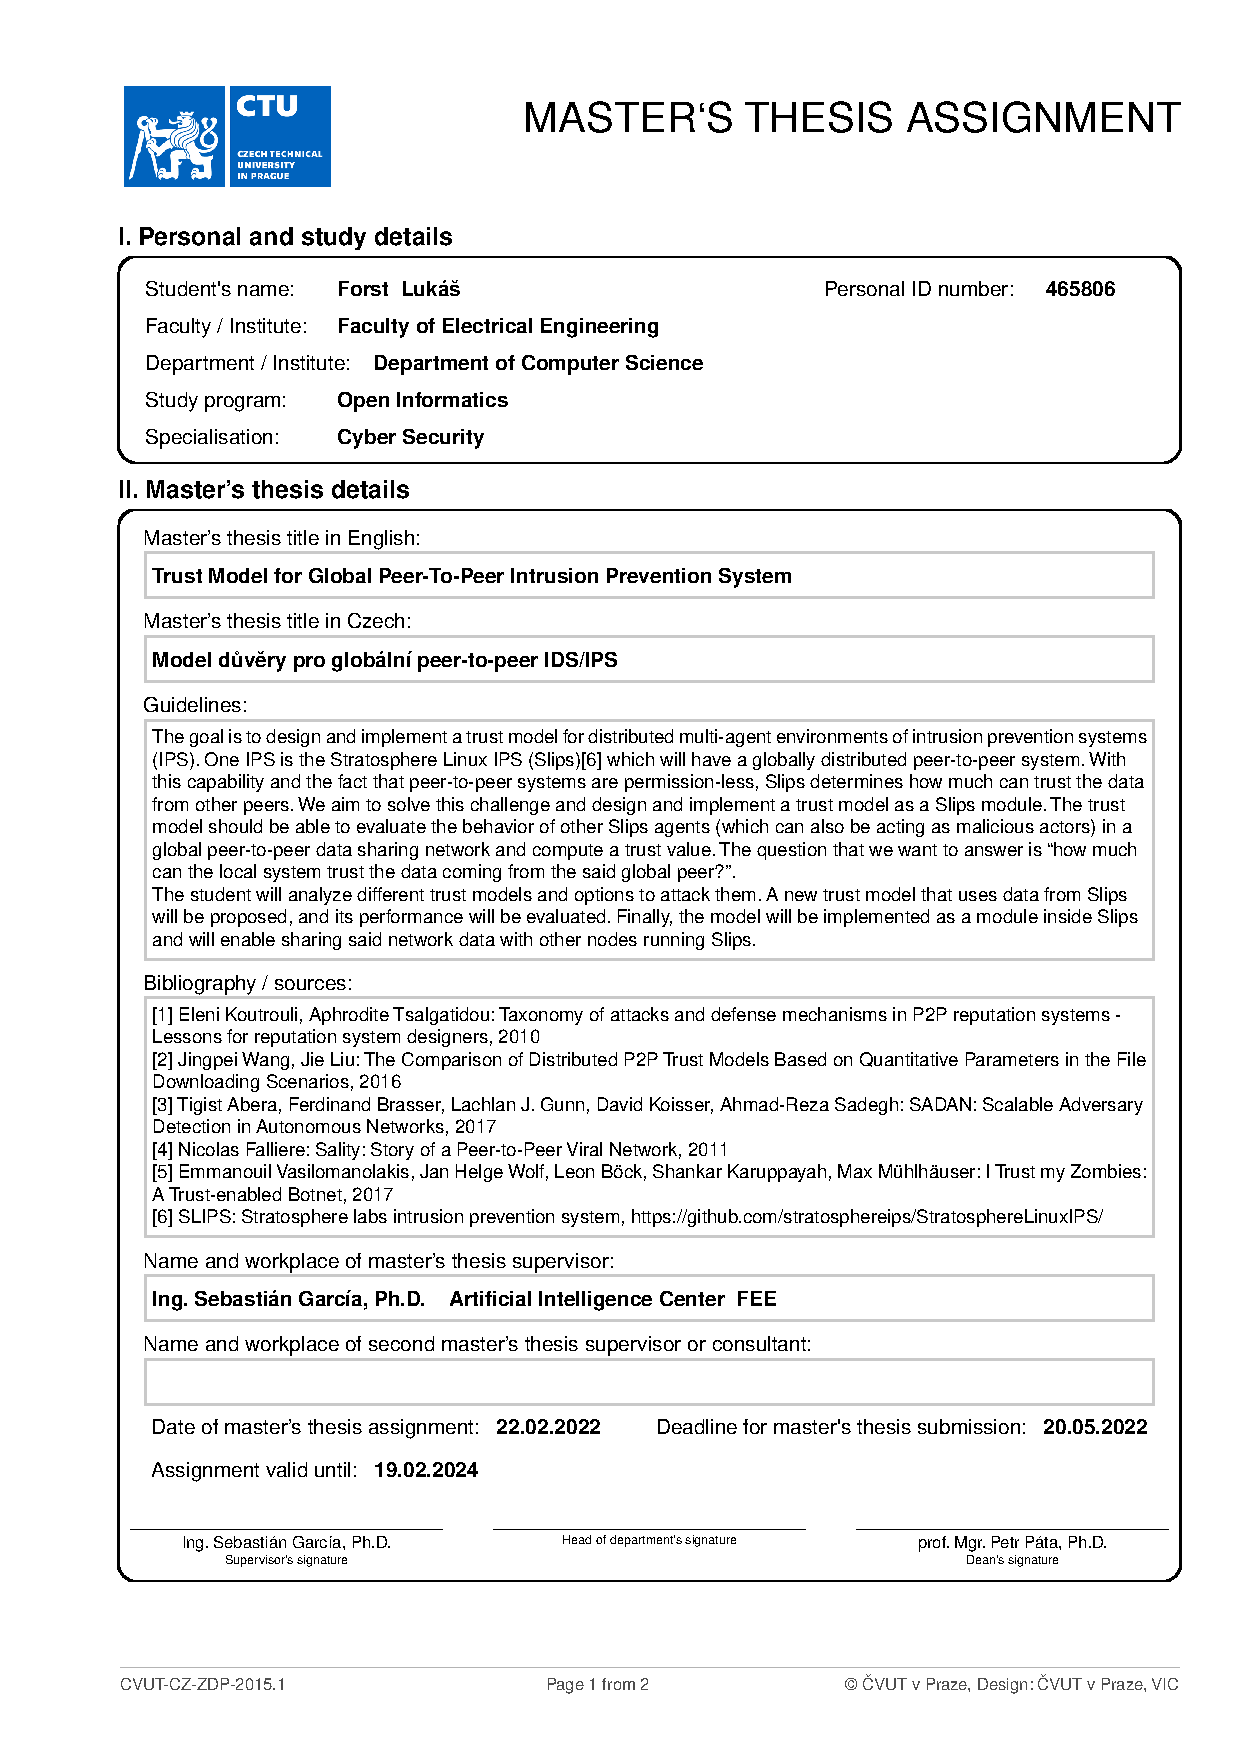
\includepdf[pages=-,scale=.8]{assets/assignment.pdf}

\section*{Declaration}
I hereby declare that the presented work has been composed solely by myself and that I have listed all sources of information used within it in accordance with the methodical instructions about ethical principles in the preparation of academic theses.

\vspace{15mm}

\begin{table}[h!]
    \centering
    \begin{tabular*}{\textwidth}{c @{\extracolsep{\fill}} c}
    \cline{1-1} \cline{2-2}
    \textit{Prague, Date}\,\,\,  & \quad\textit{Signature} \\ 
    \end{tabular*}
\end{table}

\thispagestyle{empty}

\cleardoublepage
\vspace*{\fill}

\section*{Acknowledgment}
First and foremost, I would like to thank my supervisor Sebastian Garcia for countless consultations and brainstormings and mainly for the significant amount of his time he invested in me and this thesis. Thank you.

I want to say thank you to the whole Stratosphere Research Laboratory, specifically to Veronica Valeros, Maria Rigaki, and Ondřej Lukáš, for providing me with all support I needed, for proofreading the thesis, and for guiding me through the academic world.
I'm grateful for doing this work with you and being part of the team in Stratosphere.

Finally, I must express my very profound gratitude to my parents and my whole family for providing me with unfailing support and continuous encouragement throughout my years of study and through the process of researching and writing this thesis. 

\bigskip \noindent
This accomplishment would not have been possible without you.
  
\bigskip \noindent
Thank you.
  
\bigskip \noindent
\hspace*{0.6\textwidth} 
\includegraphics[width=0.4\textwidth]{assets/signature.png}

\thispagestyle{empty}

\cleardoublepage
\newenvironment{abstractpage}
  {\cleardoublepage\thispagestyle{empty}}
  {\vfill\cleardoublepage}
\newenvironment{abstract}[1]
  {\bigskip
   \begin{center}\bfseries#1\end{center}\small\leftskip=0.5cm\rightskip=0.5cm}
  {\par\bigskip}

\providecommand{\keywords}[2]{\footnotesize\textbf{\textit{#1:}} #2}

\begin{abstractpage}
\begin{abstract}{Abstract}

Most network defense systems only rely on evidence-based knowledge about past cyberattacks, known as threat intelligence. Firewalls and intrusion prevention systems rely on the shared threat intelligence generated by other systems to prevent attacks before is too late.
Such threat intelligence is usually shared via centralized public and private blocklists where a single centralized authority, hopefully, has complete control over what is published. Such centralised system has many issues: single point of failure both technically and in trust, lack of flexibility on new data and providers, and manual trust in the providers.

To mitigate these problems, peer-to-peer networks can be used to share threat intelligence. However, because these networks are open to anyone, including malicious actors, the peers need to be able to determine who to trust and which data is better to discard.

This thesis introduce Fides. Fides is a generic trust model fine-tuned for sharing security threat intelligence in highly adversarial global peer-to-peer networks of intrusion prevention agents.
We build Fides from the lessons of other state-of-the-art trust models and optimized it for the broad spectrum of environments in the peer-to-peer network where anybody can join and leave at any time.
Apart from uncovering the behavior of any generic peer in the network, Fides is also able to identify peer's membership in organizations and utilize this knowledge for trust management.
Moreover, Fides allows administrators to filter out private data and share them only inside a single organization or with the most trusted peers. 
At the end of our work, we prove that Fides is a suitable solution for modeling trust in the global peer-to-peer networks. We show that when Fides talks to at least 25\% of peers that are part of trusted organizations, the rest of the network can be controlled by the malicious actors, and Fides is still able to determine correct threat intelligence.

\end{abstract}

\keywords{Keywords}{trust models, threat intelligence, collaborative network defense, intelligence sharing}

\vspace*{\fill}

\newpage
\begin{abstract}{Abstrakt}
    TBD \todo{add cz absrakt}
    
\end{abstract}
\keywords{Klíčová slova}{TBD1, TBD2} \todo{add cz kws}

\end{abstractpage}
\thispagestyle{empty}

\cleardoublepage

% first start roman page numbering
\pagestyle{plain}
\frontmatter 

% table of contents 
\tableofcontents
\cleardoublepage

% list of figures
%  TODO: enable this if necessary
\begingroup
\let\cleardoublepage\relax
\listoffigures
\clearpage
\endgroup

% % list of tables
\begingroup
\let\clearpage\relax
\let\cleardoublepage\relax
\listoftables
\endgroup
\cleardoublepage

 % From now on Arabic page numbering
\mainmatter

% Set header and footer styles
\pagestyle{fancy}
\fancyhf{}
\fancyhead[LE,RO]{\leftmark}
\fancyfoot[CE,CO]{\thepage}


\chapter{Introduction}
\label{ch:introduction}

% Structure of this chapter

% The why, the problem being solved
% What others did before
% The gap, what was missing
% Your proposal
% Your results
% Discussion on results/conclusions
% Your contributions

When protecting local networks, the basic firewalls and advanced Intrusion Prevention Systems (IPS)~\cite{zhang2004intrusion} rely on evidence-based knowledge about past cyberattacks, known as threat intelligence~\cite{threatintelligence}. Threat intelligence is primarily generated from the previous attacks locally or received from the remote sources.
Such sources can be, for example, public blocklists ~\cite{abuseipdb, dataplane, binarydefense} or centralized collaborative databases such as MISP~\cite{wagner2016misp} where the community collectively shares the threat intelligence.
However, all of these traditional threat intelligence sources are, in the end, controlled by the centralized authority, which has complete control over the resource and can at anytime restrict access to these valuable assets or censor what is published and what is not.
In addition, central authoriti

To limit the impact of one organization shutting down the database, we can use a peer-to-peer (P2P) model and remove the central authority and single point of failure.
In peer-to-peer networks, each peer has the same privileges and ca data are generated, shared, and consumed by each peer in the network.
Although P2P models solve the problem of a single central authority, it may introduce new problems. The most important questions to ask are: first, how much can each peer trust the threat intelligence received from other peers, given that their reliability changes? Second, how to deal with peers providing contradictory information when a single aggregated value is needed? Third, how to deal with adversarial peers that lie in many different ways?

In this thesis, we answer those questions and tackle the problem of trust relationships when sharing security threat intelligence data.
The algorithms that tackle trust relationships between multiple entities are called \textit{trust models}~\cite{wang2003trust}.
The research field of trust models is not new, and there are many existing trust models~\cite{abera2019sadan, sort, christensen2014hybrid, 1562680, huynh2006integrated, kamvar2003eigentrust, li2014design, pinyol2013computational, xiong2004peertrust}.
However, these models were primarily designed to support file sharing in peer-to-peer networks and inherently operate with different types of data. Almost no P2P system was designed to fulfill the purposes of the security community.
An exemption to them is Dovecot~\cite{dita}, a local P2P trust model designed to operate with threat intelligence data, but with the limitation that operates only in the local networks.

This thesis proposes a new trust model called \textbf{Fides}\footnote{Fides was named after the ancient goddess of trust and good faith~\cite{enwiki:1086924565}.}.
Fides is a \textit{generic} trust model fine-tuned for sharing threat intelligence in highly adversarial global peer-to-peer networks of intrusion prevention agents.
Fides was built by solving most of the problems of previous state-of-the-art trust models~\cite{sort, dita} and is optimized for a broad spectrum of networks; from local networks controlled by a single company, to public global Internet peer-to-peer networks where anybody can join and leave at any time.

Fides works with the concept of peers that belong to specific \textit{organizations} and allows administrators to pre-trust specific peers and organizations. This pre-trusting is a novel feature of Fides, representing the common criteria of security practitioners of trusting some groups or companies more than others. The comprehensive configuration options enable administrators to share data only with particular organizations. This data filtering guarantees that no privacy-sensitive intelligence is shared with peers that should not have access to it.

Fides considers many security requirements for a global P2P trust model: pre-trusted organisations, trust values depending on the service provided by the peer, asking for reputation to other peers, cold start problem of new peers, aggregation of information received, evaluation of how services were provided, adversarial peers that try to mislead others.

Fides was designed to be as modular and generic as possible, allowing other uses of its computational model for different data than threat intelligence by simply adding new evaluation methods.

Fides does not create or administer the low-level actions of the peer-to-peer network, but instead relies on a different system that performs these operations on the network layer. The system is called \textbf{Iris}. Iris was designed and developed simultaneously in the thesis by Bc. Martin Řepa~\cite{nl} and it facilitates safe and secure communications between Fides instances in the global peer-to-peer network. Communication between the two systems is done via a standard defined interface, which allows replacing the network module Iris if needed.

To interact with a real intrusion prevention system, we chose Slips~\cite{slips} and implemented a module that allows Slips to use Fides for receiving and sharing threat intelligence over the network. 
By using this shared global knowledge, Slips can prevent attacks on the local environment even before they happen by acting upon received threat intelligence from other peers in the global network.

x

The only way to evaluate our trust model was to simulate myriad complex situations. We proved that Fides could correctly uncover the peers' behavior in the network and make sensible decisions about the threat intelligence. 
Fides especially excels in the situations where it communicates with peers from trusted organizations.
Moreover, in a situation where the Fides talks to at least 25\% of pre-trusted peers, it can eventually determine correct threat intelligence no matter how other peers in the network behave and how many of them are adversarial.

\section{Thesis Structure}
\label{sec:thesis-structure}
This thesis explains the required background and describes the current state of the art in Chapter~\ref{ch:previous-work-background}.
In Chapter~\ref{ch:trust-model-design} we propose a new trust model Fides and outline how it works from the high-level perspective in Section~\ref{sec:general-overview-of-fides}.
After that, we explain problems related to gaining trust in Section~\ref{sec:cold-start-problem}.
In the following Sections~\ref{sec:attack-vectors}~and~\ref{sec:taxonomy-of-attacks} we analyze the taxonomy of attacks and the attack vectors related explicitly to the trust models and discuss how Fides defends against them.
Once we explain our design choices, we describe the entire computational model in depth in Section~\ref{sec:computational-model} and illustrate how Fides can determine trust relationships in the network by evaluating interactions between peers in the Section~\ref{sec:interaction-evaluation-strategies}.
The last part of the computational model in Section~\ref{sec:network-intelligence-aggregation} explains how Fides can aggregate threat intelligence from the network.
Chapter~\ref{ch:architecture} describes the Fides architecture and how we implemented it as a new Slips module.
In the following Chapter~\ref{ch:experiments} we propose simulations that evaluate the performance of the trust model and give a brief overview of the simulation framework that we developed alongside Fides.
Chapter~\ref{ch:results} then describes the results that we discovered in the evaluations. Finally, Chapter~\ref{ch:conclusion} concludes our results and proposes further areas of improvement for Fides. 
We also include an appendix with multiple interesting cases of evaluations discovered in Chapter~\ref{ch:results}.

\newpage
\section{List of Contributions}
\label{sec:list-of-contributions}
\noindent
The contributions of this thesis are:
\begin{itemize}
    \item Analysis of state-of-the-art trust relationships models in peer-to-peer networks.~(\ref{ch:previous-work-background})
    \item Design of Fides, a generic trust model fine-tuned for sharing security data in global adversarial peer-to-peer networks.~(\ref{sec:general-overview-of-fides})
    \item Design and implementation of multiple methods to evaluate interactions between peers that share threat intelligence data.~(\ref{sec:interaction-evaluation-strategies})
    \item A method that enables weighting and aggregation of threat intelligence from multiple peers.~(\ref{sec:network-intelligence-aggregation})
    \item A complete working reference implementation of Fides in Python.~(\ref{ch:architecture})
    \item An implementation of a Slips module that allows the use of Fides for global threat intelligence sharing.~(\ref{ch:architecture})
    \item A simulation framework for modeling any environment for Fides evaluation.~(\ref{ch:experiments})
    \item An simulated evaluation of Fides in different environments and analysis of its behavior in unfavorable situations.~(\ref{ch:results})
\end{itemize}
\chapter{Related Work}
Here we will describe what the previous work is - Dita's Dovecot, Eigen Trust, Sality, SORT etc.
Here we want to outline what the Slips is in few words.

\begin{itemize}
    \item \href{https://share.goodnotes.com/s/60IVzs1mgmuPWF54Us5eKA}{A Novel Approach to Evaluate Trustworthiness and Uncertainty of Trust Relationships in Peer-to-Peer Computing} 
    \item \href{https://share.goodnotes.com/s/7AFjiqAqJSCF1en3vt4vjS}{An Exaustive Survey of Trust Models in P2P Network}
    \item \href{https://share.goodnotes.com/s/EziqqW185BzxHxNrZ6d1MQ}{An integrated trust and reputation model for open multi-agent systems}
    \item \href{https://share.goodnotes.com/s/MRfXxmu2Lz51IqK7JODn1N}{Computational trust and reputation models for open multi-agent systems: a review}
    \item \href{https://share.goodnotes.com/s/tafBG1KUZCuYT2E7a3ucc9}{Design of Intrusion Sensitivity-Based Trust Management Model for Collaborative Intrusion Detection Networks}
    \item \href{https://share.goodnotes.com/s/YQuoXUbYADa15Hwe90sXCM}{ PeerTrust: Supporting Reputation-Based Trust for Peer-to-Peer Electronic Communities}
    \item \href{https://share.goodnotes.com/s/hRHxSYlk6wU4BEn6u9Jcyu}{SADAN: Scalable Adversary Detection in Autonomous Networks}
    \item \href{https://share.goodnotes.com/s/bXWUbVFi5qBiAdBmJ4yYAx}{SORT: A Self-ORganizing Trust Model for Peer-to-Peer Systems}
\end{itemize}
\chapter{Trust Model Design}
\label{ch:trust-model-design}
This thesis aims to design and implement a trust model for sharing threat intelligence in global peer-to-peer networks where the peers are instances of intrusion prevention systems.
The previous chapter outlined what threat intelligence is, how it is generated, and why trust relationships are essential when making decisions based on the said threat intelligence.
We described the trust models in the context of peer-to-peer networks and analyzed the notable ones.
We discovered the promising trust model SORT~,\cite{sort} which we described in section~\ref{subsec:sort}. After careful analysis, we decided to use SORT's algorithm as a base for our trust model design mainly because of its flexibility and modularity.

In this chapter, we propose a new trust model \textbf{Fides}.
Fides was named after the ancient goddess of trust and good faith Fides~\cite{enwiki:1086924565}.
The trust model utilizes modified SORT's computational model with multiple modifications and extensions that allow it to work in highly adversarial global peer-to-peer networks effectively.
Fides is a generic and heavily configurable trust model specializing in sharing threat intelligence.
However, thanks to its modular architecture, it can operate with any data, and it is not limited only to threat intelligence.

In the section~,\ref{sec:general-overview-of-fides} we describe our trust model design and explain how Fides works on a high level, the inputs and outputs, and how it behaves in which situation.

After outlining the general overview, we analyze the weaknesses of the trust models and how they apply to Fides.
First, we start with \textit{the cold start problem} in the section~\ref{sec:cold-start-problem}, which describes how peers can gain trust when they are new in the network and how Fides tackles this issue.

In the next section~\ref{sec:attack-vectors} we analyze possible attack vectors on our trust model, and then we describe the taxonomy of attacks in the next section~\ref{sec:taxonomy-of-attacks}.

Once all trust model requirements are explained, we dive deep into Fides's computational model in the next section~\ref{sec:computational-model}  and explain how it can uncover trust relationships in the network.
The following section~\ref{sec:interaction-evaluation-strategies} explains how Fides can evaluate interactions between peers and how that affects trust.
Because Fides specializes in sharing threat intelligence and integrates with Slips, in the next section~\ref{sec:network-intelligence-aggregation} we explain how Fides aggregates the weighted threat intelligence from the network.

\vspace{1cm}

\noindent
In the upcoming pages, we use the following terminology to talk about the trust model.

\begin{itemize}

\item \textbf{Target}: An identification of a resource for which is Slips able to generate threat intelligence. It can be, for example, either an IP address, domain, or hashes.

\item \textbf{Local Peer}: The unique local instance of Slips that are connected to the global P2P network and runs Fides. In equations, we use $i$ when referring to the local peer.

\item \textbf{Remote Peer}. A peer on the Internet is connected to the global Slips P2P2 network. In equations, we use $j$ when referring to the remote peer.

\item \textbf{Service Trust}: How much does Fides trust a remote peer that it provides the local peer with good service. In other words, to what extent does Fides trust a specific peer that it provides correct and valuable threat intelligence. We denote it $st$ and discuss it in detail in section~\ref{subsec:service-trust}.

\end{itemize}

\section{General Overview of Fides}
\label{sec:general-overview-of-fides}
In this section we describe how Fides work from a high level perspective. We reference chapters and sections further into the thesis that provide more information and describe particular situations and solutions in more detail.

\begin{figure}[ht!]
    \centering
    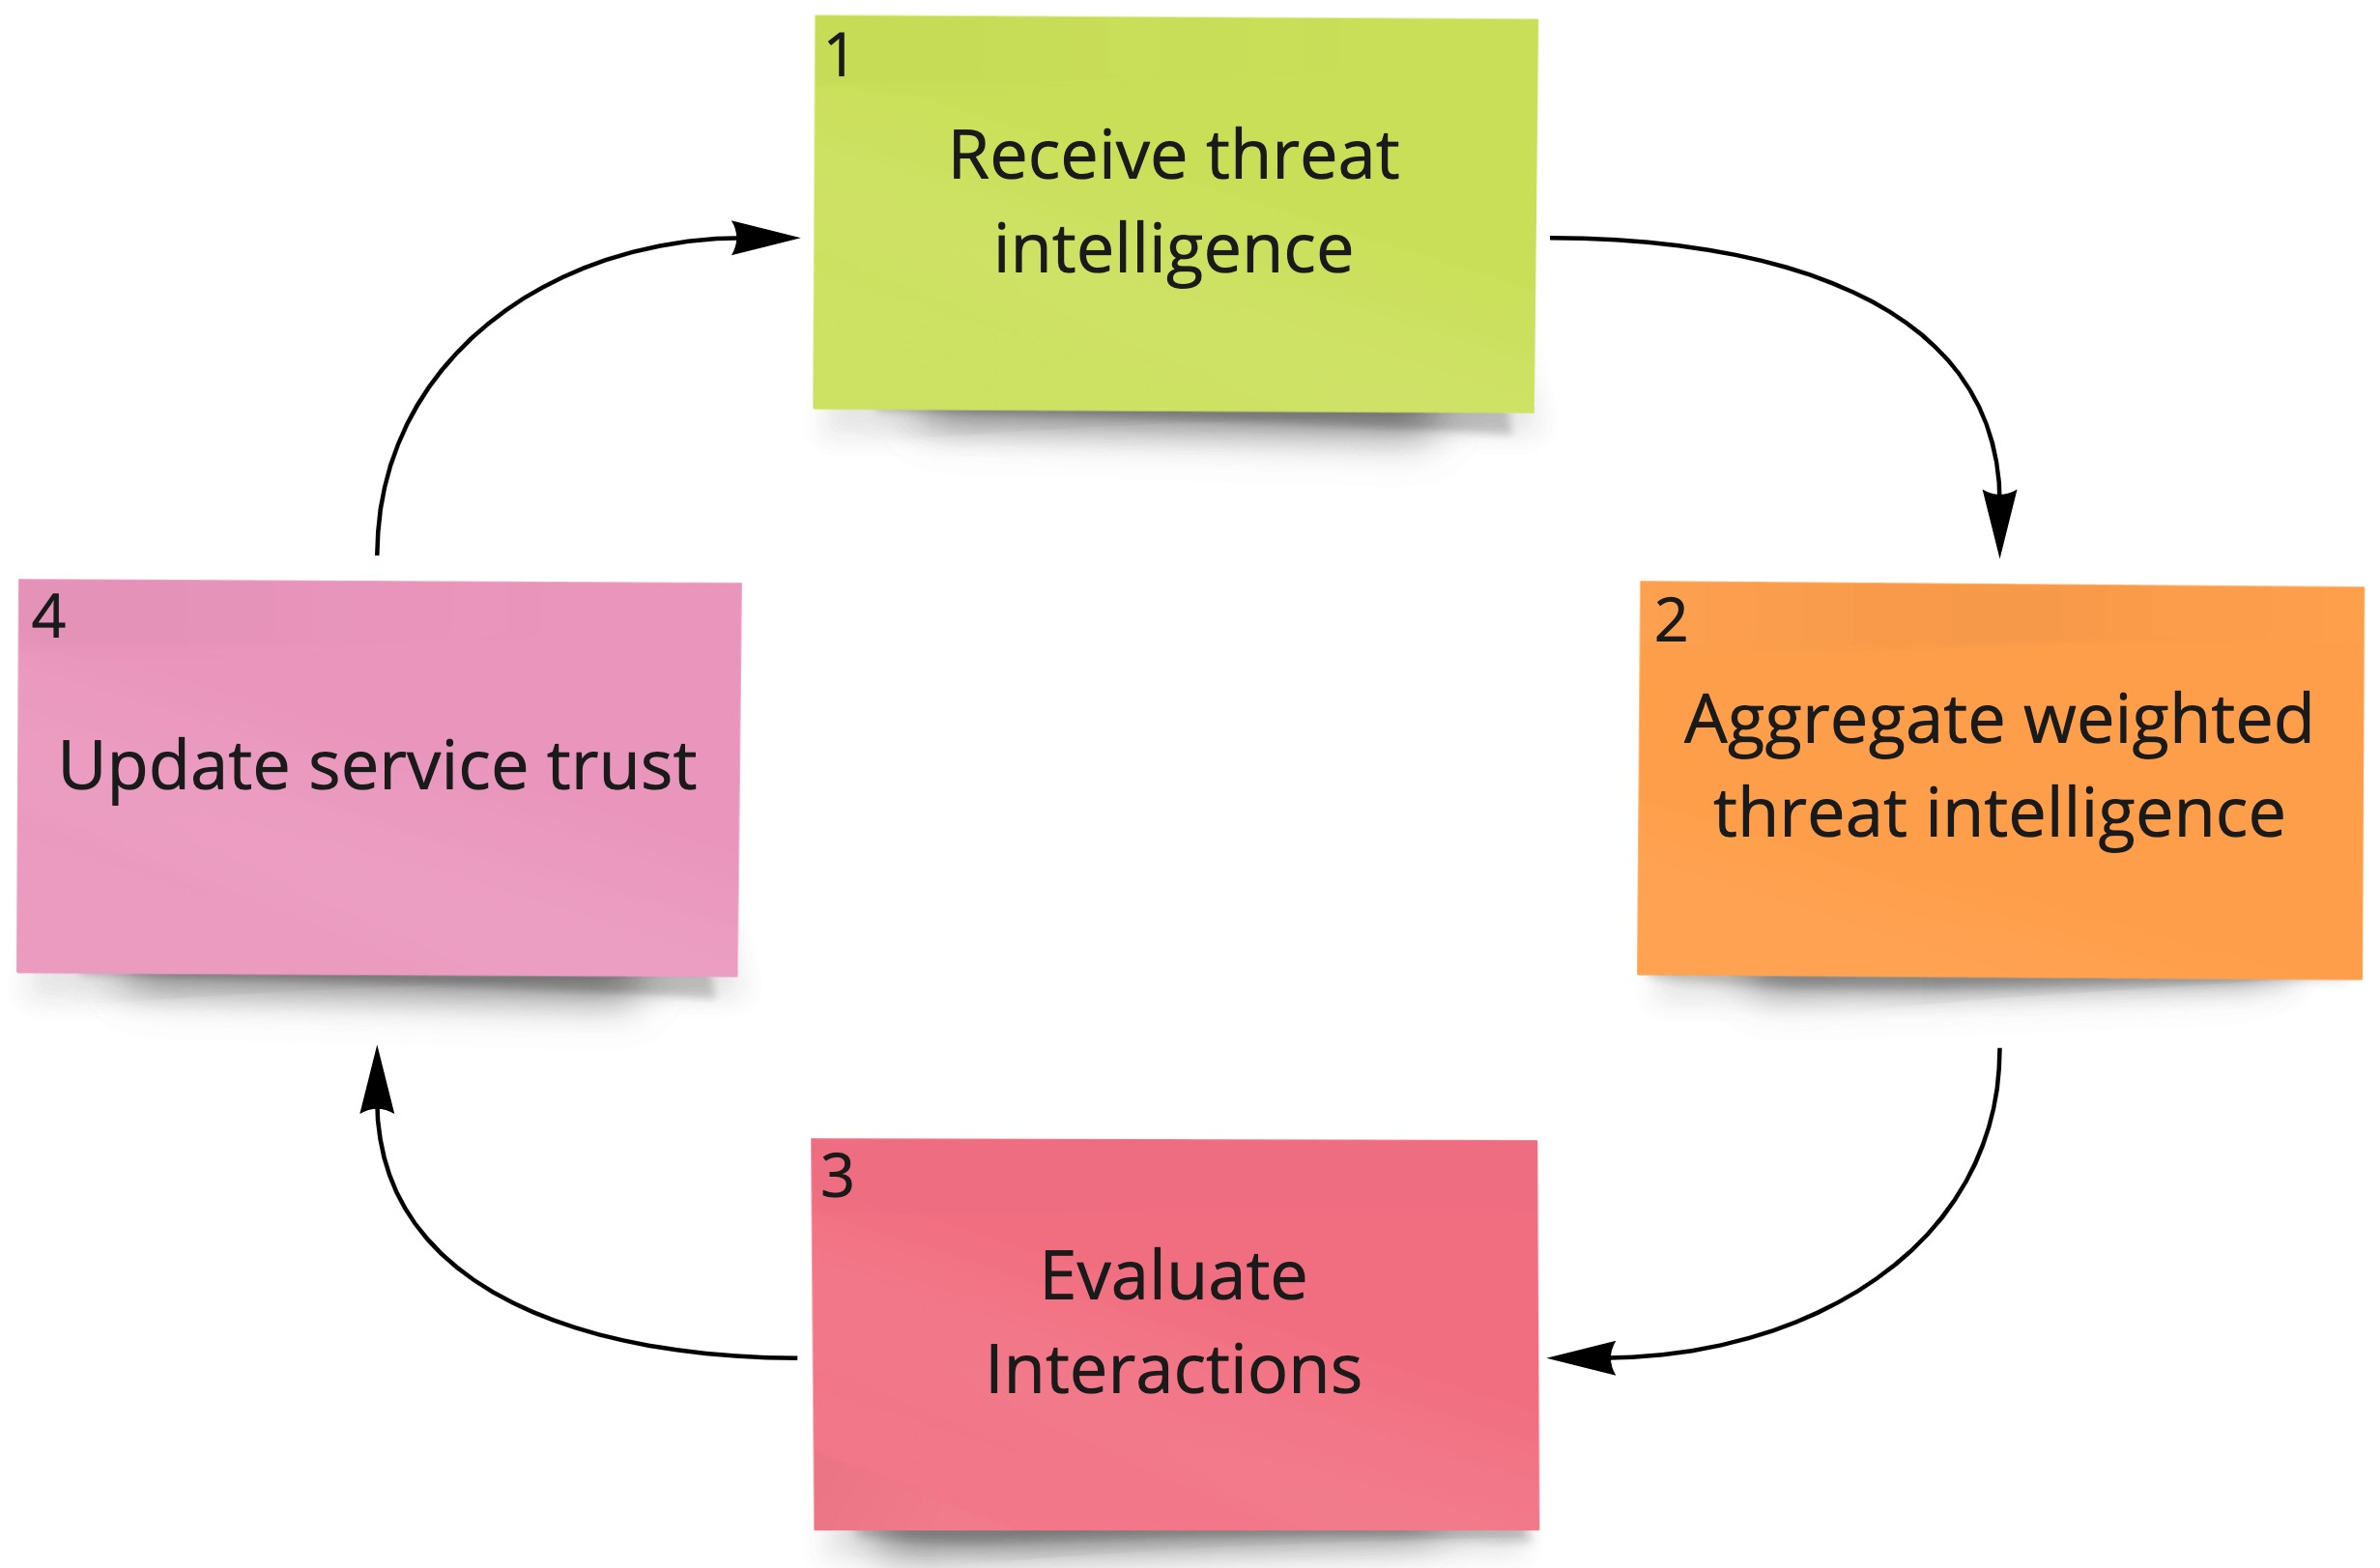
\includegraphics[width=0.75\textwidth]{assets/fides_lifecycle.jpeg}
    \caption{Generic Trust Model Life Cycle of Fides}
    \label{fig:trust-model-life-cycle}
\end{figure}

Fides operates in four general phases, which are visualized in Figure~\ref{fig:trust-model-life-cycle}.
In the first phase, a local Fides instance receives threat intelligence data from the remote peers in the network. 
How Fides receives data from the network is described in the chapter about architecture (Chapter~\ref{ch:architecture}).

In the second phase, Fides aggregates the threat intelligence data using the trust data it has for each remote peer.
In general, data from highly trusted peers have a higher impact on the final aggregated threat intelligence than the data from peers with low trust.
How does Fides do that is described in the Section~ \ref{sec:network-intelligence-aggregation}.
The aggregated threat intelligence is also sent to Slips as an output of the trust model.

In the third phase Fides evaluates the interactions with each peer.
Fides computes how much it was satisfied with threat intelligence it received from each remote peer.
This satisfaction metric has then a direct influence on the trust relationship between the local and remote peers because it is used in the next step to compute trust data. 
The evaluation process and possible interaction evaluation functions are described in detail in section \ref{sec:interaction-evaluation-strategies}.

In the last step, Fides updates trust data for each peer according to the satisfaction that is computed in step number three.
Computations that allow Fides to do that are described in detail in section \ref{sec:computational-model}.

All operations including the data flow and the communication with other peers and Slips can be found on the diagram~\ref{fig:trust-model-operational-diagram}.

\begin{figure}[h]
    \centering
    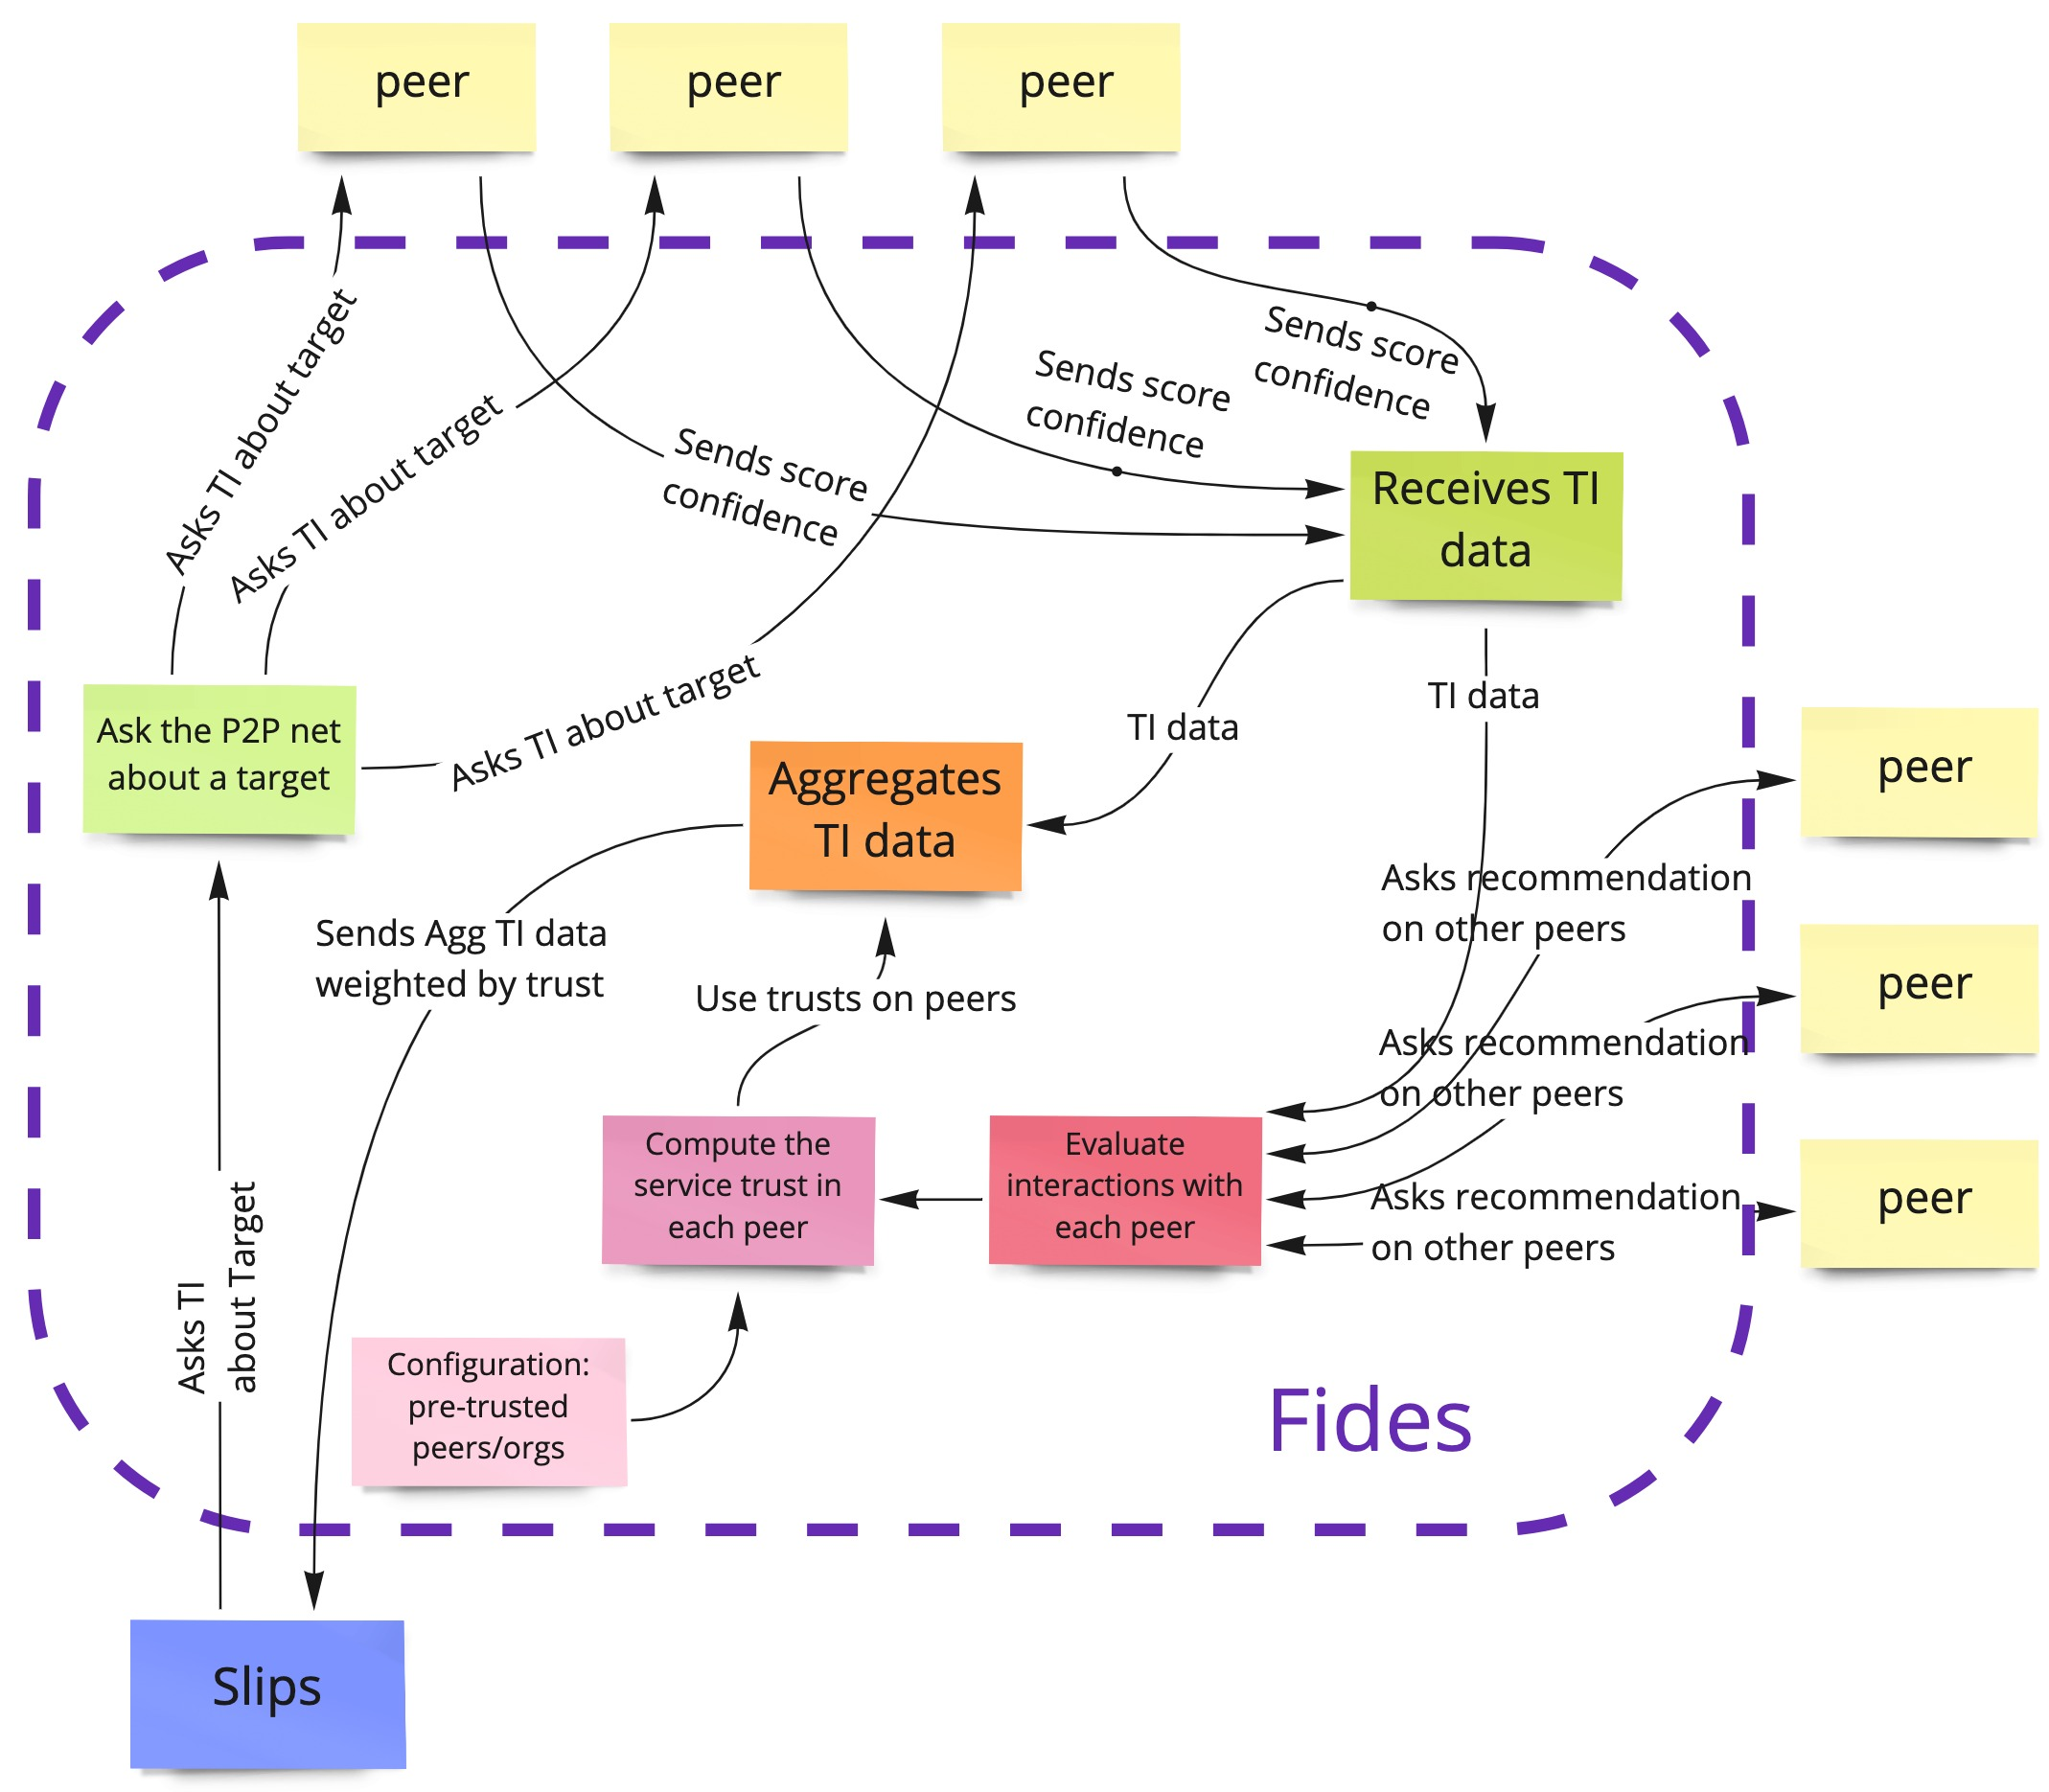
\includegraphics[width=1.0\textwidth]{assets/fides_operational_diagram.jpeg}
    \caption{Operational diagram of Fides}
    \label{fig:trust-model-operational-diagram}
\end{figure}

\section{Cold Start Problem}
\label{sec:cold-start-problem}
A dynamic and global environment such as a global peer-to-peer network is open to anyone since any peer can freely join and leave. Because of that, the local peer will encounter many other peers that were not seen before. Therefore, the trust model does not have any information about their reliability or how much it can trust them. 
New benign peers need to be \textit{somehow} trusted by the local peer in order to be a useful part of the network. However, the local peer also needs to be able to discover new malicious peers that are trying to gain its trust.

The problem of how to know something about a new entity in order to quickly work better is called the \textit{Cold Start Problem}~\cite{christensen2014hybrid}. For Fides it means how to compute a good initial trust for new unknown peers. 

We selected several solutions to this issue, which are all implemented in Fides. Fides also combines them according to a provided configuration with the aim to achieve the best result for the cold start problem with adversarial peers.

\subsection{Static Initial Trust}
\label{subsec:static-initial-trust}
In this approach, whenever the trust model encounters a new peer, it assigns a static value as an initial trust. The value is assigned by pre-choosing some third-party trust models in the configuration.

For example, in \textbf{Dovecot} trust model, every peer starts with the trust of $1$ (highest possible), and various interactions can lower the trust in the peer to $0$. In other words, the trust model considers new peers honest from the beginning, and only during this time their reputation can be lowered when they perform incorrect interactions or are discovered as a malicious peer.

On the other hand, \textbf{Sality} botnet uses \textit{goodcount} as a counter of interactions with any other peer, the higher the \textit{goodcount}, the higher trust the peer has for the local peer. The goodcount for each new peer starts with $0$. Meaning, that the botnet does not trust fresh peers at all and they can gain trust only by following the protocol which depends on a number of good interactions and time.

Static initial trust is easy to implement, but it somewhat requires assumptions about the network. If the network is considered \textit{mostly being}, it might be safe to use an initial trust of $1$, however for highly adversarial networks using an initial trust of $1$ might be dangerous and it is better to use $0$. 
On the other hand, using low initial trust and no mechanism how to gain more trust fast means, that the being peers that joined recently, don't affect the final decisions of the model even though they might have useful information about adversaries.

Static initial trust is supported by Fides as a form of fallback when no other cold start technique is used. The administrator provides a configuration that contains the initial reputation for each new peer.

\subsection{Pre-Trusted Peers}
\label{subsec:pre-trusted-peers}
In a case, when the peer-to-peer network protocol allows peers to prove their identity, or to prove membership in some group, the trust model can utilize this knowledge and assign higher or lower trust.

The network layer, designed for Slips and Fides, supports this\cite{nl} and provides a cryptographically-secure way how to identify a single peer in the network and its membership in an organization.
This allows administrators to \textit{pre-trust} peers or the whole organization - by assigning them either initial reputation or service trust directly.

The Fides configuration allows administrators to specify static initial reputation for the specific peer or for all peers from the specific organization. 
This means that whenever a new peer joins the network and it is pre-trusted, it gains the initial reputation specified in the configuration.
During this time, it interacts with the local peer and provides threat intelligence, the data are evaluated and the trust model decides how much it trusts them (assigns service trust) based on the reputation and the quality of the data. In detail is this process described in \ref{sec:interaction-evaluation-strategies}.

Another option, the administrator can use, is to enforce the service trust for the peer for the time being. This effectively means that the trust model will not evaluate any data received from the pre-trusted peer and directly assigns them service trust from the configuration. This configuration for the Fides is called \textit{enforceTrust}.

Option to pre-trust peers solves the cold start problem for specific peers and organizations, as they will start with/keep a high reputation.
Which organization or which peer to trust or not is entirely on the administrator of the trust model. The inspiration for whom to trust provides, for example, Tor and their directory authorities~\cite{torauth}.
However as the administrator needs to know the identity of the peers or organization, it does not solve the cold start problem globally for all peers.

\subsection{Recommendations}
\label{subsec:recommendations}
As the local peer might have multiple remote peers, that it \textit{trusts enough}, it could be able to utilize this relationship and ask remote peers \textit{what they think about newcomer}. 
In other words, whenever a local peer encounters a peer that wasn't seen before, they can ask for a recommendation on this peer from the local peer's most trusted remote peers.

The recommendation system introduces new attack vectors, that can be exploited by adversaries either by getting trust for the malicious peer or by lowering trust in honest peers that might have some threat intelligence about the malicious actor. 
These attacks are called \textit{bad-mouthing} and \textit{unfair praises} and we need to consider them and implement countermeasures.

Because of the possible attacks, the local peer should not solely rely on the network recommendations when computing the final service trust for the fresh peer. In case, when the recommending peers are malicious, it might skew the decisions of the local peer for the time being.
In order to solve this, when computing the final service trust for the remote peer, the local peer should take into account its own interaction with the peer as well as the received recommendations.

Moreover, the local peer should request recommendations only if it has \textit{enough} trusted remote peers, otherwise, it can expose itself to \textit{bad-mouthing} and \textit{unfair praises} attacks more easily.

\vspace{7mm}

Fides employs recommendation systems based on SORT \cite{sort} and combines it with the pre-trusted peers (\ref{subsec:pre-trusted-peers}) as well as with the static initial trust (\ref{subsec:static-initial-trust}) as a fallback when no other option is available due to constraints such as having not enough trusted peers.
The algorithm used for the recommendation system is explained in detail in section \ref{sec:computational-model}.

\section{Attack Vectors}
\label{sec:attack-vectors}
Since Fides is a trust model that computes how much to trust peers, it is potentially open to attacks from adversarial peers. Adversarial peers are peers that known how to talk the protocol and manipulate the recommendations, or threat intelligence data in order to influence the final decisions.

Adversarial peers can try to (i) send bad threat intelligence data; (ii) lie about a peer that is benign, (iii) lie about a peer that is malicious.

\subsection{Influencing Aggregated Score \& Confidence}
\label{subsec:influencing-aggregated-score-confidence}
The main output of Fides is the aggregated score and confidence of a group of reports on a target. The sequence of actions typically are (i) Slips wants to know what the P2P network thinks about target $T$. It then asks some peers (ii), and (iii) uses Fides to aggregate the scores and confidences sent by all the peers. The aggregated score and confidences are used for computing the service trust of peers and also to weight the aggregated score and confidence of the data sent by the peers.

Any attacker wants to ultimately influence these aggregated values either to make malicious IP/domain seem to be benign or another way around.
However, for that to happen, the attacker needs to gain sufficient service trust.
For more information about the aggregated threat intelligence see Section~\ref{sec:network-intelligence-aggregation}.

\subsection{Influencing Service Trust}
\label{subsec:influencing-service-trust}
Fides always computes service trust for the peers locally and does not take over the service trust computed by any other peer.
How does Fides compute service trust is described in detail in the Section~\ref{sec:computational-model}.

Malicious peers can influence the service trust value for some other remote peer in the network in the eyes of the local Fides in two situations.

Firstly, the peers can influence the service trust in a peer by manipulating their recommendation responses when the Fides encounters the peer for the first time and asks the network for the recommendations on it.
For that reason, the recommendation protocol is engaged only when the network is \textit{trusted enough} and only for the first time when the new remote peer encountered. We describe this more in detail in the Section~\ref{subsec:influencing-peers-reputation} below.

The second case when the malicious peer can indirectly influence the service trust for any other remote peer is a situation when Fides uses one of the interaction evaluation strategies that utilizes the aggregated threat intelligence (\ref{subsec:distance-based-eval}, \ref{subsec:network-intelligence-conf-high-enough}, \ref{subsec:weigh-local-opinion-with-aggregated-one}).
Because in that case, even data from malicious peers are taken in account when computing final satisfaction with the interaction for each peer so by submitting incorrect data the group of malicious peers can influence the interaction evaluation result which will lower the service trust in benign peers.

This is expected as this interaction evaluation strategy (\ref{subsec:distance-based-eval}, \ref{subsec:network-intelligence-conf-high-enough}, \ref{subsec:weigh-local-opinion-with-aggregated-one}) uses aggregated network opinion to evaluate the interactions.
Thus if the \textit{wrong} opinion is in majority, and while considering the service trust of each peer, it is taken into the account even though it is \textit{wrong}.

For that reason, the intermediate goal of an attacker is to gain the service trust of the local peer in order to have \textit{any} influence over the decisions the Fides makes.
We explore this behavior in the experiments in the Section~\ref{sec:environment-simulation} more in detail, when we let malicious peers gain the service trust at the beginning of the simulation. In addition to that, we describe how resilient Fides is to these type of attacks as a part of experiment results analysis in the Section~\ref{subsec:resilience-under-different-conditions}.

\subsection{Influencing Peers Reputation}
\label{subsec:influencing-peers-reputation}
When a new peer joins the network, Fides in some cases requests recommendations from other peers in the network.
We go into detail of this process further in Section~\ref{subsubsec:requesting-recommendation}.

Because Fides asks for the recommendation, it is possible, that one or more of the peers providing the recommendations is malicious and it provides \textit{incorrect} recommendations with a goal either to silence a benign peer or to support another malicious peer.

Even though the reputation of a peer can be skewed by the attacker, it is still able to gain \textit{correct} service trust by following the protocol and providing useful data.
The service trust equation~\ref{eq:service-trust} suggests, that  the more experience a local peer has with a remote peer, the more it ignores the initially received recommendations.
This means that the service trust will tend to converge to \textit{correct} values that do not necessarily depend on the initial recommendations and eventually will lose that information completely.
In other words, if the peer's initial reputation was \textit{incorrect} (from the ground truth point of view), it will only take the peer longer to gain \textit{correct} service trust, but eventually, it will end up with the same value as with the correct reputation value.
We talk more about the service trust and how does it behave further in the Section~\ref{subsec:service-trust}

\section{Taxonomy of Attacks}
\label{sec:taxonomy-of-attacks}
We were inspired by the thorough threat model analysis in Dovecot \cite{dita}  and based our own analysis on the same original paper from Koutrouli, Tsalgatidou \cite{KOUTROULI201247} which describes the taxonomy of different attack methods on reputation systems in peer-to-peer networks.
They classify the reputation attacks in the following categories.

\subsection{Unfair Recommendations}
\label{subsec:unfair-recommendations}
This category describes the behavior when a peer provides incorrect data.
The peer does not need to be necessarily malicious in order to do that, it can also have not enough data to make correct decisions or maybe it is missing some important information.
In the case of Fides, these types of attacks also influence service trust as well as the reputation system because the service trust depends on the initial reputation.
Moreover, the malicious peers can collude together to amplify the effect on the final computations of the trust model.

The intent of the malicious peers, in this case, is to lower someone's service trust/reputation (\textit{badmouthing attack}) or to make somebody's service trust/reputation higher (\textit{unfair praises}).
In a case of service trust, this is not possible directly, but rather by colluding with multiple high trusted peers as described in detail in Section~\ref{subsec:influencing-service-trust}.
In the case of reputation, this is possible if the malicious peer is selected as a recommender.
Fides mitigates both of these problems by asking numerous peers for their opinion (in case of service trust) and by asking only pre-selected and high trusted peers in case of recommendations.
Of course, it is not possible to eliminate the possibility of a malicious peer benign asked for the recommendations, that's why, in experiments, we simulate malicious peers as \textit{Malicious Peer} (\ref{subsubsec:malicious-peer}) behavioral patterns.
In simulations we then evaluate what network topology is needed in order for Fides not to be easily manipulated into believing the malicious peers.

\textit{Inaccurate recommendations} are a type of \textit{unfair recommendation} when an honest peer provide wrong data due to a lack of complete information.
This can happen for example because they were not attacked by the adversary (yet), and they consider them to be benign because they have no reason to see it otherwise.
Another example can be a peer that does not have the latest threat intelligence data from the black lists or other remote resources.
These peers are included in the experiments as well, we call that \textit{Confident Incorrect} (\ref{subsubsec:confident-incorrect-peer}) behavioral pattern.

Koutrouli and Tsalgatidou \cite{KOUTROULI201247} also mention \textit{Random opinions} where the peer is essentially providing random data.
We simulate this in our experiments as well, because there will be peers, in the network, that simply don't have enough information to make a good and confident decision about some target.
This is the \textit{Uncertain Peer} (\ref{subsubsec:uncertain-peer}) behavioral pattern.

Because of the nature of the Fides, which aggregates all network opinions it receives, the worst-case scenario is the situation where the attackers collude together because it amplifies their effect on the final aggregated score \& confidence.
However, our trust model uses service trust during computing the final score with confidence so, in order for attackers to influence this decision, their total service trust must be higher than the service trust of the benign peers.
This makes it harder for the adversary to overturn the decisions in their favor because it forces them to gain the service trust of all their peers.
In simulations, we have malicious peers that collude (and lie about the same targets) as well as peers that do not collude and lie about different targets.

\subsection{Inconsistent Behavior}
\label{subsec:inconsistent-behavior}
In the aforementioned Section~\ref{subsec:influencing-aggregated-score-confidence} any malicious peer needs to gain \textit{some} service trust in order to have the ability to meaningfully influence the trust model's decisions.
This leads to malicious peers that will have different behavior when they try to gain the service trust and when they provide misleading data to achieve their goals.
This behavior is equivalent to the \textit{Traitors} from \cite{KOUTROULI201247}.
Fides tries to mitigate this problem with some of the interaction evaluation strategies that compare individual threat intelligence data from a single peer to aggregated network opinion (such as \ref{subsec:distance-based-eval}).
Thanks to these strategies, even peers that gained service trust at the beginning can be eventually identified as malicious and their service trust will be lowered whenever they provide threat intelligence data that are different from the aggregated ones.

However, even the honest peers can have inconsistent behavior, mainly when they do not have enough information about IP/domains.
In experiments, we simulate this behavior for honest peers with \textit{Uncertain Peer} (\ref{subsubsec:uncertain-peer}) behavioral patterns.
For malicious peers we have a period, during which they provide correct and consistent data, allowing them to gain the service trust. 

\subsection{Identity Management Related Attacks}
\label{subsec:identity-management-attacks}
The service trust and reputation are tied to the peer's identity. 
In our case, Fides utilizes a peer's identity that was provided by the Network Layer \cite{nl}.
From the technical point of view, the identity is, in a fact, a public key, and any data the peer provides is signed with the peer's private key. Thus, we can verify that the data were provided by the owner of the private key to said public key (identity).
Moreover, any peer in our network can belong to one or more organizations that are, again, represented by their public key. 
Peer proves their membership to the organization by providing their own public key signed by the organization's private key.
The identity, as well as organization membership, is cryptographically verified by the network layer \cite{nl} and Fides does not perform any additional verification. 

\subsubsection{Impersonation}
Thanks to the data signatures and identities tied to private/public key pairs, the \textit{Impersonation} based attacks are then possible solely in cases when the attacker gained access to the private key of the peer.
Unfortunately, this type of attack is not possible to prevent completely. 
However, when the attacker gains access and starts submitting incorrect data, the Fides will start lowering service trust associated with that identity and thus eventually limiting the attacker's influence.

\subsubsection{Man-in-the-middle attack}
\textit{Man-in-the-middle attack}s are attacks when a third party is able to either intercept or manipulate the transmitted data.
From Fide's point of view, the data manipulation is not possible as the data are signed by the sender and because of the network layer \cite{nl} design and Fides never works with any data whose signature is invalid.
On the other hand, the network layer is designed in a way that peers pass messages to each other through the network \cite{nl}, so any malicious peer can choose not to pass down the message.
How this affects the propagation of messages is part of the experiments in said paper \cite{nl}.

\subsection{Whitewashing \& Sybil Attack}
\label{subsec:whitewashing-and-sybil-attack}
Due to the nature of the global peer-to-peer network, where many devices run behind NAT\footnote{Network address translation - a router mapping multiple IP addresses from the private network to a single public IP address.} or even NAPT\footnote{Network address and port translation - similar to NAT, but on the private network even the ports are used during the translation process.} and have the same IP address, the identity is not associated to an IP address.
However, this also means that any device can have multiple identities and can essentially generate new ones as time goes by.
This opens Fides to other types of attacks such as \textit{Whitewashing}, where the malicious peer drops an identity, that was discovered as malicious and its service trust dropped in $0$, and then it generates a new, fresh identity.
However, this behavior does not benefit the attacker as much as in Dovecot \cite{dita}, because Fides assigns the initial service trust $0$, instead of $1$.
In other words, Fides distrust new peers by default, so whenever a peer drops its identity and creates a new one, it starts with a service trust of $0$.

As it is not expensive to generate a new identity, it is not hard for the attacker to perform a \textit{Sybil attack}.
Sybil attack refers to a situation where a single malicious peer creates multiple identities and uses them in concert to defeat the system \cite{sybil}.
In our case, the attacker can maliciously flood the network with wrong data thus making some of the interaction evaluation strategies \ref{sec:interaction-evaluation-strategies} perform poorly.
Moreover, if the attacker is able to gain \textit{some} service trust for its malicious peers, it can effectively overtake the network and influence most of the decisions the Fides makes.
The defense against this attack is to make it \textit{computationally hard} to join the peer-to-peer network, for example by making it hard to compute peer ID or by letting peers solve some other type of computational puzzle. 

However, we did not introduce any of these measures to our system and we leave that as a part of future work (\ref{sec:future-work}) in Section~\ref{subsec:possible-mittigation-of-sybil-attack}. 

\section{Computational Model of Fides}
\label{sec:computational-model}
This section describes how Fides to whom and how much it can trust other remote peers.
Our trust model expresses trust in a specif peer with metrics called \textit{service trust}.
Service trust is a value that describes how much the local peer can trust a \textit{specific} remote peer. 

In the following pages, we describe the process top-down starting with the most important parts - service trust - and then breaking it down into bits.
Note that there are two main ideas behind most of the equations. 

The first one, is that we want to robustly capture the average behavior of the peers. In order to do that, we will be computing the average behavior of the peers and then approximating the deviations from said behavior.

Secondly, we will be comparing and weighing first-hand experience with the remote experience. 
First-hand experience is what happened between local and remote peers during the time they interacted. This can be, for example, threat intelligence sharing, file-sharing, or the results of the recommendation protocol.
Remote experience is what happened between one remote peer and another remote peer. In other words, first-hand experience for peer $j$ are actions between $j$ and $z$. Whenever $j$ shares information about these actions with peer $i$, for $i$ it is a remote experience.

\vspace{0.5cm}

\noindent
Table~\ref{tab:notation-computational-model} describes the most important notation we use in the following sections.

\begin{table}[ht]
\centering
\begin{tabular}{ c | m{20em} }
 $i$ & local peer, instance of Fides \\
 \hline
 $j$ & remote peer somewhere on the internet \\
 \hline
 $st_{i, j}$ & service trust - how much $i$ trusts $j$ that it provides good service \\
 \hline
 $r_{i, j}$ & $i$'s reputation value about $j$ \\
 \hline
 $rt_{i, j}$ & $i$'s recommendation trust about $j$ \\
 \hline
 $sh_{i, j}$ & size of $i$'s service history with $j$ \\
 \hline
 $s^{k}_{i, j}$ & $i$'s satisfaction value with interaction with peer $j$ in window $k$\\
 \hline
 $w^{k}_{i, j}$ & weight of $i$'s interaction with $j$ in $k$ \\
 \hline
 $f^{k}_{i, j}$ & fading effect of $i$'s interaction with $j$ in $k$ \\
\end{tabular}
\caption{Fides Computational Model Notation}
\label{tab:notation-computational-model}
\end{table}

\subsection{Service Trust}
\label{subsec:service-trust}
As outlined previously, service trust $st_{i, j}$ is a value that describes how much peer $i$ trusts that remote peer $j$ will provide a \textit{good service}~\cite{sort}.
We compute the $st_{i, j}$ in the equation~\ref{eq:service-trust} by weighing local experience with peer's $j$ service, with the reputation $j$ got from the network when it was first seen by $i$.
The used weight is the size of the service interaction history $sh_{i,j}$ to global maximal history size $sh_{max}$.

\begin{equation}
\label{eq:service-trust}
    st_{i,j}=\frac{sh_{i,j}}{sh_{max}} \cdot \left(cb_{i,j} - \frac{1}{2} ib_{i,j} \right) +\left(1-\frac{sh_{i,j}}{sh_{max}}\right) \cdot r_{i,j}
\end{equation}

Equation~\ref{eq:service-trust} implies that the more interaction there was between peers $i$ and $j$, the bigger impact on $st_{i,j}$ it has. 
In other words, the more $i$ and $j$ interact the less $i$ relies on the reputation that $i$ computed from the values provided by the network, at the time when $j$ was seen for the first time by the peer $i$.

\subsection{Local Experience for Service Trust}
The first part of the equation \ref{eq:service-trust} contains \textit{competence belief} - $cb_{i,j}$, and \textit{integrity belief} - $ib_{i,j}$.
Both values are based solely on the history of the interactions that the peer $i$ experienced with the peer $j$.

\subsubsection{Competence Belief}
\textit{Competence belief} represents how much did peer $j$ satisfied local peer $i$ with the past interactions. We measure it as an average of interactions from the past~\cite{sort}.

\begin{equation}
\begin{split}
    cb_{i,j} &= \frac{1}{\beta_{cb}} \sum_{k=1}^{sh_{i, j}} s_{i,j}^{k} \cdot w_{i,j}^{k} \cdot f_{i,j}^{k} \\
    \beta_{cb} &= \sum_{k=1}^{sh_{i, j}} s_{i,j}^{k} \cdot w_{i,j}^{k}
\end{split}
\end{equation}

It holds that $0 \leq cb_{i,j} \leq 1$ and where $s^{k}_{i,j}$ is the evaluation of the interaction in window $k$, $w^{k}_{i, j}$ is the weight of the interaction (how important it was) and $f^{k}_{i,j}$ is the fading effect of that interaction. We describe $s^{k}_{i,j}$, $w^{k}_{i,j}$ and $f^{k}_{i,j}$ in Section~\ref{subsec:interaction-satisfaction}. 
$\beta_{cb}$ is the normalization coefficient that ensures that $cb_{i, j}$ stays within the interval of $0 \leq cb_{i,j} \leq 1$.

\subsubsection{Integrity Belief}
\textit{Integrity belief} $ib_{i,j}$ is a level of confidence in the predictability of future interactions~\cite{sort}. It is measured as a deviation from the average behavior $cb_{i,j}$.
Therefore, $ib_{i,j}$ is calculated as an approximation to the standard deviation of interaction parameters~\cite{sort}.

\begin{equation}
\begin{split}
    ib_{i,j} &= \sqrt{\frac{1}{sh_{i,j}} \sum_{k=1}^{sh_{i,j}}\left(s_{i,j}^{k} \cdot w_{i,j}^{\mu} \cdot f_{i,j}^{\mu} - cb_{i,j}\right)^{2}} \\
    f_{i,j}^{\mu} &= \frac{1}{sh_{i, j}} \sum_{k=1}^{sh_{i,j}} f^{k}_{i,j} \\
    w_{i,j}^{\mu} &= \frac{1}{sh_{i, j}} \sum_{k=1}^{sh_{i,j}} w^{k}_{i,j}
\end{split}
\end{equation}

It holds that $0 \leq ib_{i,j} \leq 1$.
The more consistent behavior peer $j$ has, the lower the $ib_{i,j}$ is. Consistency is a highly desired property as the local peer then has more precise estimates about the future behavior of the remote peer.

\subsection{Interaction Satisfaction}
\label{subsec:interaction-satisfaction}
$s^{k}_{i, j}$ is $i$'s satisfaction value with interaction with peer $j$ in window $k$~\cite{sort}.
We outlined before, that each interaction between two peers is evaluated, $s^{k}_{i, j}$ is a result of this evaluation of a single interaction between peers $i$ and $j$.
Because our trust model is generic, the evaluation function can be implemented differently for different data.
How did we design it and implemented it for threat intelligence is described in the Section~\ref{sec:interaction-evaluation-strategies}.

However, even with the computed interaction satisfaction value, not all interactions are the same. 
Some interactions are more important than others. 
Moreover, because peers can change their behavior, most recent interactions should be more important than the interactions that happened a long time ago.
That is why we include the weight of the interaction and the fading effect.

\subsubsection{Weight of the Interaction}
Because each interaction is different and its importance is different, we have $w^{k}_{i,j}$ that measures the importance~\cite{sort}.
The weight belongs to interval $0 \leq w^{k}_{i,j} \leq 1$ and Fides implements it as a discrete function of interaction type. 
For example, the weight of interaction when a remote peer shares the threat intelligence is higher than when the remote peer requests threat intelligence.


\subsubsection{Fading Effect}
\label{subsubsec:fading-effect}
Fading effect $f^{k}_{i,j}$ determines \textit{"how much does the algorithm forget"} as the algorithm prefers most recent interactions over past interactions and thus $f^{k}_{i,j}$ reduces the weight of the past interactions~\cite{sort}. 
$f^{k}_{i,j}$ is a \textit{non-increasing function} of interaction and time or an index of said interaction in history.

The actual implementation of the fading effect depends on the data the trust model is processing.
For example, SORT implements it as a decreasing linear function $f^{k}_{i,j} = \frac{k}{sh_{i,j}}, 1 \leq k \leq sh_{i,j}$~\cite{sort}.
However, in our case and after multiple iterations, we decided not to forget the interactions that the model remembers and rather have all interactions with the same impact.

\begin{equation}
    f^{k}_{i,j} =1
\end{equation}

\noindent
The way Fides computes $f^{k}_{i,j}$ might be changed in the future and implemented as a function of time, we discuss this in more detail as a part of the future work in Section~\ref{sec:future-work}.

\subsection{Reputation and Recommendations}
In order to mitigate the cold start problem outlined in Section~\ref{sec:cold-start-problem} and in the cases when there are no or few interactions between $i$ and $j$, the algorithm relies on $r_{i,j}$ - \textit{reputation value}~\cite{sort}.
$r_{i,j}$ is the second part of the service trust equation~\ref{eq:service-trust} that introduces \textit{remote experience} to the service trust.

The \textit{reputation} value is computed from the \textit{recommendations} received from the remote peers. This value represents what remote peers think about another remote peer. However, this value is calculated by the local peer with respect, to how much it trusts each peer, that provided the recommendation.
When the local peer $i$ encounters remote peer $j$ for the first time and it does not have any data about its trustworthiness, $i$ can request recommendations on peer $j$ from $i$'s most trusted peers.
We denote a set of remote peers, that provided the recommendations as $T_{i}$.

\subsubsection{Requesting a Recommendation}
\label{subsubsec:requesting-recommendation}
The recommendation system built into Fides cannot be used in every scenario.
Because of the sensitive nature of the environment, the trust model was designed for, there are cases when it is dangerous to ask for recommendations.
This is mainly the case when there are \textit{not enough} peers that are \textit{trusted enough}.

SORT requests recommendations every time it encounters a new peer. The set of recommending peers is created by taking all known peers and selecting the ones that have higher than average service trust.
However, those can also be peers with trust as low as $0.001$. In a sensitive environment, which the peer-to-peer network of IPS definitely is, we do not want to get recommendations from peers, that have low trust at all.
Moreover, given the nature of Slips, we decided to combine a recommendation system based on SORT with static initial trust~(\ref{subsec:static-initial-trust}) and with pre-trusted peers~(\ref{subsec:pre-trusted-peers}).
This approach provides a more robust basis for a trust-sensitive environment and it helps us to mitigate the cold start problem~(\ref{sec:cold-start-problem}).

If the peer is part of a pre-trusted organization or it is pre-trusted itself, it inherits the configured reputation - $r_{i, j}$ from the configuration.
In this case, Fides does not engage the recommendation protocol at all, because the peer already has reputation $r_{i,j}$ assigned from the configuration and it was \textit{recommended} by the administrator.
Moreover, the administrator can choose if this value is \textit{frozen}, or not. 
\textit{Frozen Service Trust} configuration means, that the peer $j$ has in eyes of $i$ \textit{static service trust} $st_{i, j}$ - it will never change and whatever data peer $j$ sends to $i$ will not influence the $st_{i,j}$.
On the other hand, when this configuration is not selected, the peer's service trust is going to change during the time when it communicates with the local instance according to the data and interactions it provides.

In the case where the peer is not pre-trusted, Fides evaluates if it has \textit{enough} well-trusted peers that can be trusted to provide the correct recommendation. This value as well as a number of maximal peers used for recommendation is configurable.
In addition, the administrator can enforce that for the recommendation protocol, only the pre-trusted peers or the peers from pre-trusted organizations are used.

\subsubsection{Recommendation Response}
A single recommendation response from peer $z \in T_{i}$ about giving the recommendation to peer $i$ about peer $j$ contains the following data.
\begin{itemize}
    \item $cb_{z,j}$, $ib_{z,j}$ - summary of $z$'s interactions with $j$, competence belief and integrity belief
    \item $sh_{z,j}$ - service history size, number of the interactions between $z$ and $j$ - the more interactions they had, then the $z$'s recommendation has more credibility
    \item $r_{z, j}$ - summary of recommendations that $z$ received on $j$
    \item $\eta_{z,j}$ - number of peers that provided recommendations for $j$ when $j$ was new to $z$ and their recommendation was used to compute $r_{z,j}$
\end{itemize}

$cb_{z,j}$, $ib_{z,j}$ are included in the recommendation in order to provide a view on what does $z$ think about $j$.
$sh_{z,j}$ and $\eta_{z,j}$ are included to indicate how much experience with $j$ does $z$ actually have. To determine to which extent is the $z$ sure about correctness of $cb_{z,j}$, $ib_{z,j}$, $r_{z, j}$ in the recommendation.
And also to protect the $z$'s recommendation trust in $i$'s eyes, if $cb_{z,j}$, $ib_{z,j}$, $r_{z, j}$ values are wrong, because $i$ inspects $sh_{z,j}$ and $\eta_{z,j}$ and does not penalize $z$ that much, if the history size or the number of original recommender are low.

\subsubsection{Computing Reputation}
\label{subsubsec:computing-reputation}
When the local peer receives all recommendations, it computes the reputation value $r_{i,j}$ as a weighed expected local experience ($ecb_{i,j}$, $eib_{i,j}$ - estimates about competence and integrity) from the remote peers with their remote experience ($er_{i,j}$ - estimate about reputation of said peer).

\begin{equation}
\label{eq:reputation-value}
\begin{split}
    r_{i, j}=\frac{\lfloor\mu_{sh}\rfloor}{sh_{max}} \cdot \left(ecb_{i,j}-\frac{1}{2} eib_{i, j}\right) + \left(1-\frac{\lfloor\mu_{sh}\rfloor}{sh_{max}}\right) \cdot er_{i,j}
\end{split}
\end{equation}

\noindent
The weight, used in the Equation~\ref{eq:reputation-value}, is the average of history sizes in all recommendations to $sh_{max}$, maximal interactions history size. 
We calculate $\mu_{sh}$ as follows.
\begin{equation}
    \mu_{sh} = \frac{1}{|T_{i}|} \sum_{z \in T_{i}} sh_{z, j}
\end{equation}
\noindent
Again, we are weighing local experience to remote experience. However, in this case, it is local for the remote peers that provided the recommendations.

\subsection{Remote Local Experience}
\label{subsec:remote-local-experience}
Similarly, when we compute the service trust in Equation~\ref{eq:service-trust}, we need to get competence and integrity belief.
However, while creating reputation value in \ref{eq:reputation-value} where the values are coming from the remote peers, we are trying to estimate those values received from the network.
For that reason, we call them \textit{estimated competence belief} - $ecb_{i,j}$ and \textit{estimated integrity belief} - $eib_{i,j}$.

\subsubsection{Estimated Competence Belief}
$ecb_{i,j}$ is estimation about competence belief made by $i$ about $j$. 
This value is computed from the received recommendations in combination with $rt_{i,z}$ - a \textit{recommendation trust} that $i$ has about $z$.
Similarly, as for service trust, we have a normalization coefficient $\beta_{ecb}$ that moves the resulting data to the correct interval.
It holds that $0 \leq ecb_{i,j} \leq 1$.

\begin{equation}
\label{eq:estimated-competence-belief}
\begin{split}
    ecb_{i,j} &= \frac{1}{\beta_{ecb}} \sum_{z \in T_{i}} \left(rt_{i, z} \cdot sh_{z, j} \cdot cb_{z, j}\right) \\
    \beta_{ecb} &= \sum_{z \in T_{i}} \left(rt_{i, z} \cdot sh_{z, j}\right)
\end{split}
\end{equation}

\noindent
Recommendation trust $rt_{i, z}$ is described in detail in Section~\ref{subsec:recommendation-trust-metric}.

\subsubsection{Estimated Integrity Belief}
Following the $ecb_{i,j}$, $eib_{i,j}$ is estimation about the integrity belief made by $i$ about $j$.
The equation is almost similar, but we use $ib_{z,j}$ instead of $eb_{z,j}$.
This means that normalization coefficient $\beta_{eib} = \beta_{ecb}$.

\begin{equation}
\label{eq:estimated-integrity-belief}
\begin{split}
    eib_{i,j} &= \frac{1}{\beta_{eib}} \sum_{z \in T_{i}} \left(rt_{i, z} \cdot sh_{z, j} \cdot ib_{z, j}\right) \\
    \beta_{eib} &= \sum_{z \in T_{i}} \left(rt_{i, z} \cdot sh_{z, j}\right)
\end{split}
\end{equation}

\subsection{Remote Remote Experience}
Going back to Equation~\ref{eq:reputation-value} from Section~\ref{subsubsec:computing-reputation}, we use \textit{estimated reputation value} - $er_{i,j}$.
This value represents information that was created by the peers, that are remote even for remote peer $j$. 
Essentially making it information that came from the \textit{second ring of trust} - from acquaintances of an acquaintance.

\begin{equation}
\label{eq:estimated-reputation}
\begin{split}
    er_{i,j} &= \frac{1}{\beta_{er}} \sum_{z \in T_{i}} \left(rt_{i, z} \cdot \eta_{z, j} \cdot r_{z, j}\right) \\
    \beta_{er} &= \sum_{z \in T_{i}} \left(rt_{i, z} \cdot \eta{z, j}\right)
\end{split}
\end{equation}

\subsection{Recommendation Trust Metric}
\label{subsec:recommendation-trust-metric}
Recommendation trust - $rt_{i,z}$ - is another metric that a peer calculate and store. It expresses how much does $i$ trust that $z$ provides \textit{good recommendations}.
Even though one could theoretically use service trust $st_{i, z}$ for this,
we have another trust metric because there are peers that can provide very good data (service), but they are surrounded by bad peers or the other way around.
This also gives us the ability to have specialized nodes in the network, that serves as a peers registry for organizations - a single node that only provides recommendations on peers.

We calculate the recommendation trust in a similar way as the service trust and reputation, but we use recommendation competence belief $rcb_{i, z}$, recommendation integrity belief $rib_{i,z}$ and reputation $r_{i, z}$.
This time, we use the weight $rh_{i,z}$, which is the size of the history of the recommendations provided by $z$ to $i$, and $rh_{max}$, the maximal size of said history.

\begin{equation}
\label{eq:recommendation-trust}
\begin{split}
    rt_{i, z} = \frac{rh_{i,z}}{rh_{max}} \left(rcb_{i,z} - \frac{1}{2} rib_{i, z} \right) + \left(1 - \frac{rh_{i,z}}{rh_{max}} \right) r_{i,z}
\end{split}
\end{equation}

\subsubsection{Recommendation Competence and Integrity Belief}
\label{subsubsec:recommendation-competence-integrity-belief}
Similar for interactions, we use three different parameters for calculating the $rcb_{i, z}$ and $rib_{i,z}$. 
We use satisfaction $rs^{x}_{i, z}$, weight $rw^{x}_{i, z}$ and the fading effect $rf^{x}_{i, z}$. 
The parameters have the same background as described in the Section~\ref{subsec:interaction-satisfaction}, but in this case, they are connected to recommendations instead of service.
We calculate $rcb_{i, z}$ as follows:

\begin{equation}
\begin{split}
    rcb_{i, z} &= \frac{1}{\beta_{rcb}} \sum_{x = 1}^{rh_{i, z}}\left(rs_{i,z}^{x} \cdot rw_{i, z}^{x} \cdot rf_{i,z}^{x}\right) \\
    \beta_{rcb} &= \sum_{x = 1}^{rh_{i, z}}\left(rw_{i, z}^{x} \cdot rf_{i,z}^{x}\right)
\end{split}
\end{equation}

\noindent
And for recommendation integrity we compute $rib_{i, z}$ as:
\begin{equation}
    rib_{i, z} = \sqrt{\frac{1}{rh_{i, z}} \sum_{x=1}^{rh_{i,z}} \left(rs_{i,z}^{x} \cdot rw_{i, z}^{\mu} \cdot rf_{i,z}^{\mu} - rcb_{i,z}\right)^{2}}
\end{equation}

\noindent
One more time, the computational model is trying to approximate average behavior in recommendations - $rcb_{i,z}$ - and then the deviation from such behavior - $rib_{i,z}$.

Fading effect $rf^{x}_{i, z}$ has similar properties as the fading effect for service trust described in Section~\ref{subsubsec:fading-effect}. It is a non-increasing function of a number of recommendations or a time. 
For the recommendations, Fides implements it exactly the same as for the service interactions.

\begin{equation}
    rf^{x}_{i, z} = 1
\end{equation}

\subsubsection{Evaluating Received Recommendation}
As outlined in the Section~\ref{subsubsec:recommendation-competence-integrity-belief}, in order to evaluate a particular recommendation from remote peer $z$, we have satisfaction, weight, and the fading effect. 
We calculate the recommendation satisfaction $rs^{x}_{i,z}$ by comparing values from $z$'s recommendation $r_{z,j}$, $cb_{z,j}$, $ib_{z,j}$, with values that are the results of the the recommendation algorithm.
In other words, we compare each recommendation, with the aggregated values - $er_{i,j}$, $ecb_{i,j}$ and $eib_{i,j}$. This gives us an estimate of how off was the peer $z$'s recommendation from the final result of the recommendation algorithm.

\begin{equation}
\begin{split}
    rs^{x}_{i,z} = \frac{1}{3} \left[ \left(1-\frac{\left|r_{z, j} - er_{i,j}\right|}{er_{i,j}}\right) + \right. \\
    \left(1 - \frac{\left|cb_{z, j} - ecb_{i, j}\right|}{ecb_{i, j}}\right) + \\
    \left. \left(1 - \frac{\left|ib_{z, j} - eib_{i, j}\right|}{eib_{i, j}}\right)\vphantom{\frac{1}{2}}\right]
\end{split}
\end{equation}

We calculate the weight of recommendation $rw^{x}_{i,z}$ as a weighed sum of the proportion of the size of the service history between $z$ and $j$ with maximal service history size. And a number of peers that provided the initial reputations $\eta_{z,j}$ divided by a maximal number of possible recommending peers.
\begin{equation}
    rw^{x}_{i,z} = \frac{\lfloor\mu_{sh}\rfloor}{sh_{max}} \cdot \frac{sh_{z, j}}{sh_{max}} + \left(1 - \frac{\lfloor\mu_{sh}\rfloor}{sh_{max}}\right) \cdot \frac{\eta_{z,j}}{\eta_{max}}
\end{equation}


\section{Interaction Evaluation Strategies}
\label{sec:interaction-evaluation-strategies}
In order to determine what remote peers are providing valuable data and what peers are are not, the local peer needs to be able to evaluate each interaction it had with the remote peer.
In general, there are two options how to approach this - either by designing evaluation that is protocol aware (meaning, that it understands the protocol and the data that are two peers sharing with each other), or by having an evaluation function that does not need to understand the protocol and can be used for any data.

We choose to implement both approaches and they are described in the following sections. In order to evaluate which strategy is better in what scenarios, we designed and run many simulations - their results are described in chapter \ref{ch:experiments}. 
We will use notation from table (\ref{table:interaction-eval})  when referring to peers and their interactions.\todo{maybe do not use S and C when referring to score and confidence as we use "s" for satisfaction}

\begin{table}[h!]
\centering
\begin{tabular}{ c | m{20em} }
 $i$ & local peer \\
 \hline
 $j$ & remote peer \\
 \hline
 $T$ & target of network intelligence, domain or IP address \\
 \hline
 $k$ & evaluation window \\
 \hline
 $s^{k}_{i, j}$ & $i$'s satisfaction value with interaction with peer $j$ in window $k$\\
 \hline
 $S^{k}_{j, T}$ & score computed by the peer $j$ about target $T$ in window $k$ \\
 \hline
 $C^{k}_{j, T}$ & confidence, how much is the score correct \\
 \hline
 $S^{k}_{T}$ & aggregated score from all threat intelligence reports in window $w$ for target $T$ \\
 \hline
 $C^{k}_{T}$ & aggregated confidence
\end{tabular}
\caption{Interactions Symbols}
\label{table:interaction-eval}
\end{table}

\subsection{Evaluate all interactions with the same value}
\label{subsec:same-eval-for-all-interactions}
The strategy, that does not need to understand underlying data, their semantics nor their structure.
It is a naive approach when the trust model uses the same satisfaction value for all data it received. It does not check, if the data make sense (for example when all other peers but one are reporting that the IP address is malicious) and assigns all peers same satisfaction value $s^{k}_{i, j}$. 
The idea behind this algorithm is that when the peers are interacting for a longer time or have more interactions, they're more trustworthy.

This approach is for example used by the botnet \textbf{Sality} or by the \textbf{Dovecot} trust model. Fides implements it as $EvenTIEvaluation$ strategy with configurable satisfaction value and administrator can use this strategy if they see it as the most optimal.

The disadvantage of this approach is, that we do not penalize remote peers when they provide wrong data, because the evaluation method does not care nor understand the underlying data.
Because of that and in a case when the adversary gains the service trust of the model by following the protocol for longer time, it may significantly influence the aggregated score as the adversary has higher trust then other remote peers. If this happens, there is no way to automatically downgrade adversary's service trust.

\subsection{Use aggregated network intelligence for evaluation}
\label{subsec:distance-based-eval}
Because Fides is designed for the sharing and aggregating threat intelligence and understands the protocol that is being used, we can utilize this and penalize peers that are providing local peer with incorrect data.
The interaction evaluation is performed at the end of the threat intelligence sharing process, at that point, Fides already aggregated data and decided what is the aggregated network score and confidence. 
Thus, we can utilize aggregated values and use it as a base line. Then we compare it against every each remote peer's threat intelligence we received. This evaluation strategy is implemented in the Fides a as a $DistanceBasedTIEvaluation$.

% TODO: here we need to set correct indexes, because k-th interaction between local and peer i is not necessarily the same number as for the peer i+1 -> that means that for S_a we will need another number
% TODO: we need to move this to another section and to describe what is score and what is confidence
Suppose, that remote peer $j$ provided data about target $T$ to local peer $i$ in window $k$. Provided data consist of score and confidence - ($S^{k}_{j, T}$, $C^{k}_{j, T}$). Where score,  $-1 \leq S^{k}_{j, T} \leq 1$, indicates if the target is malicious ($-1$) or begin ($1$). The confidence $0 \leq C^{k}_{j, T} \leq 1$ on the other hand indicates, how much is the peer sure about its assessment of $S^{k}_{j, T}$.

In order to evaluate interaction between the local peer $i$ and remote peer $j$ we need to compute satisfaction value $s^{k}_{i, j}$. 
It holds that  $0 \leq s^{k}_{i, j} \leq 1$ - where $1$ means peer $i$ was satisfied with the interaction.
% TODO: [?] this equation can be more robust, we can for example, compute standard deviation from the S^{k}_{T} and then compare each S to nearest second quantile -> that way the equation is more robust
\begin{equation}
s^{k}_{i, j} = \left(1 - \frac{|{S}^{k}_{T} - S^{k}_{j, T}|}{2} \cdot C^{k}_{j, T}\right) \cdot C^{k}_{T}
\end{equation}

Where $S^{k}_{T}$ is final score aggregated across the reports from the peers, $C^{k}_{T}$ is aggregated confidence.

The problem in this evaluation algorithm are the situations when the aggregated confidence $C^{k}_{T}$ is close to $0$. In this case the algorithm will penalize all peers for providing any threat intelligence as the final $s^{k}_{i, j}$ is close to $0$. Another issue with this approach is that when a single honest peer has a unique information about an IP address or domain, which is significantly different then what other peers have, it is automatically penalized for not sharing the same opinion as the other peers. However, if the peer is trusted enough, it has higher impact on the aggregated value and it is not penalized too much.

\subsection{Use network intelligence only if the confidence is high enough}
\label{subsec:network-intelligence-conf-high-enough}
In order to compensate for the low confidence $C^{k}_{T}$ and penalizing all peers in algorithm explained in \ref{subsec:distance-based-eval}, this evaluation strategy considers $C^{k}_{T}$ value and employs  $DistanceBasedTIEvaluation$ only when the  $C^{k}_{T}$ is \textit{"high enough"}. In this case \textit{"high enough"} means higher then configured value by the Slips administrator - ${CT}$.
In a case when  $C^{k}_{T} < {CT}$, the algorithm fall backs to using $EvenTIEvaluation$, because it is not possible to distinguish between \textit{"good"} and \textit{"bad"} network intelligence due to low confidence of the decision. 
This strategy is implemented in Fides under the name $ThresholdTIEvaluation$.
What should be the correct value for $CT$ from configuration is subject to evaluation in the simulations in chapter \ref{ch:experiments}.

\begin{algorithm}
\caption{$ThresholdTIEvaluation$}\label{alg:threshold-ti-evaluation}
\begin{algorithmic}[1]
\State ${CT} \gets configuration$ \Comment{configuration provided by the administrator}
\If{$C^{k}_{T} < {CT}$}
	\State $s^{k}_{i, j} \gets EvenTIEvaluation()$
\Else
    \State $s^{k}_{i, j} \gets DistanceBasedTIEvaluation()$
\EndIf
\end{algorithmic}
\end{algorithm}

\subsection{Use local threat intelligence to evaluate network intelligence}
\label{subsec:use-local-threat-to-evaluate}
This approach uses similar equation for computing satisfaction value outlined in \ref{subsec:distance-based-eval}. However, the input is different - instead of comparing remote peer's ($j$ ) threat intelligence ($S^{k}_{j, T}$, $C^{k}_{j, T}$) to aggregated intelligence ($S^{k}_{T}$, $C^{k}_{T}$), we compare it to the threat intelligence of the local ($i$) Slips instance - ($S^{k}_{i, T}$, $C^{k}_{i, T}$). Thus the evaluation is following:

\begin{equation}
s^{k}_{i, j} = \left(1 - \frac{|{S}^{k}_{i, T} - S^{k}_{j, T}|}{2} \cdot C^{k}_{j, T}\right) \cdot C^{k}_{i, T}
\end{equation}

This approach is useful when local peer has enough information about the target, but it wants to verify the behavior of the remote peers.
To determine whether they are sending data that are somewhat correct. This strategy is implemented in Fides with name $LocalCompareTIEvaluation$.

\subsection{Weight local opinion with aggregated one}
\label{subsec:weight-local-opinion-with-aggregated-one}
Another implemented strategy combines \ref{subsec:distance-based-eval} and \ref{subsec:use-local-threat-to-evaluate} and mixes them using weight $w$, provided from the configuration.
This is good approach when the the Slips or the network has a lot of data on the target. It evaluates interactions with what local instance thinks and what the network opinion is.
What the correct mixture is is subject to simulations and configuration from the administrator.

\begin{equation}
\begin{split}
    s^{k}_{i, j} = w &\cdot \left(1 - \frac{|{S}^{k}_{i, T} - S^{k}_{j, T}|}{2} \cdot C^{k}_{j, T}\right) \cdot C^{k}_{i, T} + \\
    (1-w) &\cdot \left(1 - \frac{|{S}^{k}_{T} - S^{k}_{j, T}|}{2} \cdot C^{k}_{j, T}\right) \cdot C^{k}_{T}
\end{split}
\end{equation}

\noindent
In Fides implemented as the $WeightedDistanceToLocalTIEvaluation$.

\subsection{Utilize all available data in evaluation}
The goal of this strategy is to evaluate the received data with as much confidence as possible while having fully automatic process without the administrator's configuration.
In order to do that, we combine all previous strategies into one, where we utilize all available information into a single $s^{k}_{i, j}$ value.

We introduce new variables here - $w_{0}, w_{1}, w_{2}$ - which are essentially weights of the particular strategies. These weights are based on the confidence, that the strategy has in its own decision.
Note, that there is a hierarchy and order matters. 
In our case we decided to prefer decisions coming from strategy \ref{subsec:distance-based-eval}, then we add data from the \ref{subsec:use-local-threat-to-evaluate} and if the final decision still does not have confidence of $1$, we add static value configured by the administrator (noted as $S_{C}$). 
The last part - $S_{C}$ - simulates static strategy described in \ref{subsec:same-eval-for-all-interactions} and is set by the Slips administrator.\todo{should we use min or the detailed version?}

\begin{equation}
\label{equation:strategies-weights}
\begin{split}
    w_{0} &= {C}^{k}_{T} \\
    w_{1} &= min(1 - {C}^{k}_{T}, {C}^{k}_{i, T}) \\
    w_{2} &= 1 - w_{0} - w_{1}
\end{split}
\end{equation}
The weights $w_{0}, w_{1}, w_{2}$ in \ref{equation:strategies-weights}, are designed to gather as much confidence as possible. $p_{0}$ is confidence of the aggregated network data, essentially saying how much is the network sure about the given score. 
$p_{1}$ is the confidence coming from the local IPS and the $p_{2}$ is the remaining confidence to $1$.

When we have the weights, we can compute final $s^{k}_{i, j}$ where we use strategies - $w_{0} \cdot \ref{subsec:distance-based-eval}$, $w_{1} \cdot \ref{subsec:use-local-threat-to-evaluate}$ and $w_{2} \cdot \ref{subsec:same-eval-for-all-interactions}$. 
\begin{equation}
\begin{split}
    s^{k}_{i, j} &= \\
    &w_{0} \cdot \left[\left(1 - \frac{|{S}^{k}_{T} - S^{k}_{j, T}|}{2} \cdot C^{k}_{j, T}\right) \cdot C^{k}_{T}\right] + \\
    &w_{1} \cdot \left[\left(1 - \frac{|{S}^{k}_{i, T} - S^{k}_{j, T}|}{2} \cdot C^{k}_{j, T}\right) \cdot C^{k}_{i, T}\right] + \\
    &w_{2} \cdot S_{C}
\end{split}
\end{equation}

\noindent
This strategy is implemented in Fides under a name $MaxConfidenceEvaluation$.


\section{Network Intelligence Aggregation}
\label{sec:network-intelligence-aggregation}
Fides is a trust model designed for global peer-to-peer networks of Slips instances.
It is designed to support Slips in detecting malicious actors on the network and enables threat intelligence sharing between peers of Slips instances.
Because Slips was designed to be as modular as possible, Fides is effectively running as a module that provides aggregated threat intelligence to Slips. 
In other words, Fides provides a view of what the network thinks about some threat intelligence target. This is necessary so Slips can have a unique \textit{view} of the network on a specific Threat Intelligence.
Fides needs to aggregate elements of threat intelligence from remote peers into a single value that is then presented to Slips.

Fides needs to say that some reports are better than others, based on the service trust the local peer has in the remote peer (previously computed as $st^{k}_{i, j}$).
Thus Fides needs to weigh every report based on this trust and come up with an aggregated score $S^{k}_{T}$.
Apart from the aggregated score, Fides needs to compute the aggregated confidence $C^{k}_{T}$ that expresses how confident $i$ is about the aggregated score $S^{k}_{T}$ that was computed in the previous step.

Once aggregated, the computed score and confidence ($S^{k}_{T}$, $C^{k}_{T}$) are sent to Slips to report data on target $T$.
Apart from sending to Slips, these same values can be also used to evaluate the interaction of the remote peers, depending on the selected interaction evaluation strategy. We describe this more in depth in section~\ref{sec:interaction-evaluation-strategies}.

We designed and implemented two different functions for aggregating threat intelligence and computing $S^{k}_{T}$ alongside with $C^{k}_{T}$.
Both of them are implemented in Fides under their respective names and which method performs better under what circumstances is a subject of the experiments in chapter~\ref{ch:experiments}.

\subsection{AverageConfidenceTIAggregation}
\label{subsec:AverageConfidenceTIAggregation}

In this method, the aggregated score $S^{k}_{T}$ is the sum of $S^{k}_{j, T}$, which is the score sent by each peer $j$ about target $T$ in time window $k$; weighed with the normalized service trust that $i$ computed for peer $j$, denoted $wst^{k}_{i, j}$. The sum is done over the set of remote peers that provided a report to $i$ for $T$ in time window $k$, denoted $R^{k}_{i, T}$. We calculate it in equation~\ref{eq:ti_aggregation_score}.

\begin{equation}
\begin{split}
    S^{k}_{T} &= \sum_{{j}\in R^{k}_{i, T}} wst^{k}_{i, j} \cdot S^{k}_{j, T}
\end{split}
\label{eq:ti_aggregation_score}
\end{equation}

\noindent
The normalized service trust $wst^{k}_{i,j}$ used as weight is computed as:

\begin{equation}
\begin{split}
    wst^{k}_{i,j} &= \frac{1}{\sum_{{j}\in R^{k}_{i, T}} st^{k}_{i, j}} \cdot st^{k}_{i, j} \\
\end{split}
\label{eq:normalized_service_trust_ti_aggregation}
\end{equation}

\noindent
Equation~\ref{eq:normalized_service_trust_ti_aggregation} estimates the percentage that the service trust on $j$ $st^{k}_{i, j}$ has relative to the total sum of service trust received by $i$ for all peers, for this target $T$, in time window $k$.

We compute the aggregated confidence $C^{k}_{T}$ for this strategy as:

\begin{equation}
\begin{split}
    C^{k}_{T} &= \frac{1}{|R^{k}_{i, T}|} \cdot \sum_{{j}\in R^{k}_{i, T}} st^{k}_{i, j} \cdot C^{k}_{j, T}
\end{split}
\end{equation}

\noindent
Which is an average, overall the peers that sent to $i$ a report on $T$ in time window $k$, of the weighted confidence sent by peer $j$ on target $T$ on time window $k$. The weight is done by the service trust that $i$ has on $j$ on time window $k$.


\subsection{WeightedAverageConfidenceTIAggregation}
\label{subsec:WeightedAverageConfidenceTIAggregation}

This strategy uses equation~\ref{eq:ti_aggregation_score} to compute the aggregated score $S^{k}_{T}$ similarly to the $AverageConfidenceTIAggregation$ in section~\ref{subsec:AverageConfidenceTIAggregation}.
However, the way how this strategy calculates $C^{k}_{T}$ is different. 
Instead of using the service trust $st^{k}_{i, j}$ to determine the correct trust in the confidence $C^{k}_{j, T}$ submitted by peer $j$ and then diving it by the number of peers, it uses the normalized service trust $wst^{k}_{i,j}$ computed in equation~\ref{eq:normalized_service_trust_ti_aggregation} that already contains the weight of the peers in the final decision.

\begin{equation}
\begin{split}
    C^{k}_{T} &= \cdot \sum_{{j}\in R^{k}_{i, T}} wst^{k}_{i,j} \cdot C^{k}_{j, T}
\end{split}
\end{equation}
\chapter{Architecture}

\section{one arch1}

\section{one arch2}
\chapter{Experiments}
\label{ch:experiments}
We designed a single and comprehensive experiment that simulates a real-world usage of Fides. This chapter describes how we set up an environment that allows us to run experiments and simulate real-world situations in the peer-to-peer network where the peers communicate and share threat intelligence.

In section~\ref{sec:sampling-threat-intelligence} we describe how we sample threat intelligence shared by the peers.
In the following section~(\ref{sec:peers-behavioral-patterns}), we list different types of peers in the network, what is their goal, and how they behave.
Section~\ref{sec:environment-simulation} then describes how we designed the environment and what are the inputs for the simulation itself.
The last section~(\ref{sec:experiments-evaluation}) presents how we evaluate each scenario and explains the vital simulation indicators.

\section{Sampling Threat Intelligence}
\label{sec:sampling-threat-intelligence}
Threat intelligence, which is being shared on the peer-to-peer network and is aggregated by Fides, is generated inside Slips by various modules.
Each module provides a score on its own and Slips aggregates these evaluations into a single value. 
This means, that threat intelligence is computed as a sum of independent random variables and that tends to follow the normal distribution. 
For that reason, we sample threat intelligence values from the normal distribution.

As peers have different behavior, we will sample the threat intelligence provided by them every time when they are asked for it.
We will characterize the peer's behavior by the threat intelligence it provides, with respect to the baseline, and the ground truth of the target being benign or malicious.

As described in the previous chapters, threat intelligence consists of a \textit{score} and the \textit{confidence} in that score.
We use the notation $\mu_{s}$ for the mean threat intelligence score and $\sigma_{s}$ for the standard deviation of the score. 
Similarly, we use $\mu_{c}$ for mean confidence and $\sigma_{c}$ for the standard deviation of the confidence. 

Fides also in some cases employs a recommendation protocol, so in the simulations, the peers might be asked to provide recommendations about other peers.
They will follow their behavioral strategy when providing the data. 
Recall the recommendation description from section \ref{subsec:recommendations}. A single recommendation response contains $cb_{k,j}$, $ib_{k,j}$, $sh_{k,j}$, $r_{k,j}$ and $\eta_{k,j}$. 
We will be sampling those from the normal distribution as well with the corresponding pairs of $(\mu_{cb}, \sigma_{cb})$, $(\mu_{ib}, \sigma_{ib})$, $(\mu_{sh}, \sigma_{sh})$, $(\mu_{r}, \sigma_{r})$ and $(\mu_{\eta}, \sigma_{\eta})$.
Every peer will provide recommendations based on his behavioral strategy with respect to the ground truth.



\section{Peer's Behavioral Patterns}
\label{sec:peers-behavioral-patterns}
For the sake of the experiments, every peer will follow one of the chosen behaviors.
We identified multiple different behavioral patterns for the benign as well as for the malicious peers.
Every behavior is different and is defined by the $(\mu, \sigma)$ for every data we sample and by the intent the peer has in the network.
Most of the behavior depends on the baseline, which is the ground truth for any target in the system - if it is benign or malicious.
We note baseline score as $S_{B} \in \{-1, 1\}$, where $S_{B} = -1$, means the target is malicious and $S_{B} = 1$ means the target is benign.


\subsection{Confident Correct Peer}
\label{subsubsec:confident-correct-peer}
This behavior corresponds to an honest peer that provides correct data according to the baseline. 
Meaning, that if the target (domain/IP address that we have threat intelligence for) is benign, the peer with \textit{confident correct} behavior will provide threat intelligence that says that the target is benign. 
Moreover, the peer will provide the data with high confidence.

The very same thing applies to the situation when this peer is asked to provide a recommendation for any other peer. 
The provided recommendation will reflect the real behavior of said peer and it will indicate high confidence in the recommendation.
This peer has the \textit{ideal} behavior as its data are useful and correct.
The table \ref{tab:confident-correct} describes the data used for sampling the threat intelligence this peer provides.

\begin{table}[!ht]
    \centering
    \begin{tabular}{c|c|c|c}
        type & notation & $\mu$ & $\sigma$ \\
        \hline
        score & $\mu^{cc}_{s}$ & $S_{B} \cdot 0.9$ & $0.1$ \\
        confidence & $\mu^{cc}_{c}$ &  $0.9$ & $0.1$ \\
    \end{tabular}
    \caption{Confident Correct Behavior}
    \label{tab:confident-correct}
\end{table}

\subsection{Uncertain Peer}
\label{subsubsec:uncertain-peer}
This behavior simulates peers that do not have enough information to provide reasonably good data, but they are benign and honest with their behavior.
The peer can provide essentially any score but with very low confidence in said score.

\begin{table}[!ht]
    \centering
    \begin{tabular}{c|c|c|c}
        type & notation & $\mu$ & $\sigma$ \\
        \hline
        score & $\mu^{up}_{s}$ & $0.0$ & $0.8$ \\
        confidence & $\mu^{up}_{c}$ &  $0.3$ & $0.2$ \\
    \end{tabular}
    \caption{Uncertain Peer Behavior}
    \label{tab:uncertain-peer}
\end{table}

\subsection{Confident Incorrect}
\label{subsubsec:confident-incorrect-peer}
The peer with this behavior is confident about their data and the threat intelligence, but their threat intelligence is wrong.
However, this peer is still benign and is making honest mistakes.
This strategy simulates peers that were not attacked by a malicious device and they consider it benign because they do not have any information indicating malicious intent.
Thus, whenever the peer is asked to provide threat intelligence, it responds with a score that is opposite of the baseline and with a high confidence value.

\begin{table}[!ht]
    \centering
    \begin{tabular}{c|c|c|c}
        type & notation & $\mu$ & $\sigma$ \\
        \hline
        score & $\mu^{ci}_{s}$ & $-S_{B} \cdot 0.8$ & $0.2$ \\
        confidence & $\mu^{ci}_{c}$ &  $0.8$ & $0.2$ \\
    \end{tabular}
    \caption{Confident Incorrect Behavior}
    \label{tab:confident-incorrect}
\end{table}


\subsection{Malicious Peer}
\label{subsubsec:malicious-peer}
The malicious peer is going to provide wrong threat intelligence intentionally to achieve their goal of influencing the trust decisions of the local peer. 
The sampling data are the same as for the \textit{confident incorrect} (section~\ref{tab:confident-incorrect}) behavior, but the difference is that the malicious peer is providing misleading data intentionally.

This behavior simulates knowledgeable adversaries that are able to follow the Fides's protocol and their goal is to influence decisions of the local trust model.
The adversaries can be either trying to \textit{bad-mouth} or provide \textit{unfair praises}.
In our case, it does not matter why they do that, but rather the fact, that they do that intentionally and that they are providing the opposite of the baseline score with the high confidence.

We decide to design an attacker, that is trying to hide in the data and it is not providing score $\{-1, 1\}$ with the confidence of $1$ all the time, but rather uses a distribution that is close to these values.
The reason is that if the model sees that there is a peer that provides $\{-1, 1\}$ with high confidence all the time, it would be very easy to detect and penalize this behavior.

\begin{table}[!ht]
    \centering
    \begin{tabular}{c|c|c|c}
        type & notation & $\mu$ & $\sigma$ \\
        \hline
        score & $\mu^{m}_{s}$ & $-S_{B} \cdot 0.9$ & $0.1$ \\
        confidence & $\mu^{m}_{c}$ &  $0.9$ & $0.1$ \\
    \end{tabular}
    \caption{Malicious Behavior}
    \label{tab:malicious-peer}
\end{table}



\section{Environment Simulation}
\label{sec:environment-simulation}
It is important in the simulations to also simulate time. This is because the trust model depends on when peers join the network and when they decided to lie or not. It is also because new peers are subject to recommendation requests, but only when they are new.

Time in the simulations is measured in \textit{clicks}. 
The local instance of Fides performs a single action and receives responses from other peers in the network in exactly \textit{one click}. 
For example, this is the series of events that happen in a \textit{single click}. Fides asks the network for threat intelligence, receives the responses, aggregates network opinion, and evaluates the interactions with peers.
Another series of events happening in a \textit{single click} is the actions of  recommendation protocol: a new peer joins the network, Fides asks for the recommendation for  a new peer, collects the responses, computes the reputation, and evaluates the received recommendations.
What is the relation between real time and the \textit{clicks} depends solely on the network layer, mostly on the speed of messages convergence described in-depth in \cite{nl}.

In order to simulate the environment, we have multiple parameters that correspond to the expectations of how does the peer-to-peer network looks like.
We start with the \textbf{number of peers in network} that simulates the size of the network and how many different peers can appear during the whole simulation.

The network anatomy is another parameter for the simulation, where define what \textbf{percentage of peers} are using \textbf{what strategy} that were described in the section \ref{sec:peers-behavioral-patterns}. 
In other words, how many peers in the network are adversarial and how many of them are benign.

Another parameter is \textbf{number of targets} (IP addresses and DNS domains) that will be used when the Fides will be requesting the network threat intelligence.
For each target, we know the label (malicious and benign) and we will be sampling threat intelligence that came from the local Slips instance. 
The local threat intelligence will be sampled from parameters of one of the strategies described in \ref{sec:peers-behavioral-patterns} - confident correct, uncertain or confident incorrect - which is yet another parameter that describes how the local Slips behave.

For each remote peer, we select one of the behaviors from \ref{sec:peers-behavioral-patterns}, \textbf{the number of peers for each behavior} is determined by the configuration of the simulation.
We also determine if the peer is pre-trusted or if it is a member of the pre-trusted organization. \textbf{Percentage of pre-trusted peers} is again configurable.
Next we determine the \textbf{time} (in $clicks$), when the peer is going to \textbf{join the network}. This allows us to evaluate the recommendation part of Fides, because if the peer joins late, Fides requests recommendations from the other peers which can lead to further problems if the recommending peers are adversarial.

If the strategy selected in the previous step is malicious (with behavior \ref{subsubsec:malicious-peer}), we determine for \textbf{how many targets} is the peer going to \textbf{lie} about.
This allows us to also simulate highly advanced attacker that lies only selectively for the targets that they control.
It is not rational for the attacker to lie about targets that are not known to them as they do not gain any advantage from that. On the contrary, if they do not lie, they gain more trust which they can use to further influence the local decisions. 

The last simulation parameter is how many \textit{clicks} are left at the beginning, for the pears to gain the initial trust.
This means that in that initial time period, malicious peers will behave like confident (\ref{subsubsec:confident-correct-peer}), in order to gain initial trust, and after that, they will switch to their own malicious behavior (\ref{subsubsec:malicious-peer}).
This allows us to evaluate how fast is the trust model able to determine that the peer, with existing service trust, is malicious

\section{Experiments Evaluation}
\label{sec:experiments-evaluation}

An important part of the experiments is how to evaluate what Fides setup \textit{(interaction evaluations, threat intelligence aggregation)} is better in which scenario. We will be measuring two performance metrics that are relevant for each situation.

\subsection{Target Detection Performance Metric}
\label{subsec:target-detection-performance-metric}
This first metric, $tdp$, measures performance of the target detection.
We compute $tdp$ in Equation~\ref{eq:target_detection_metric} as an average distance between the ground truth for the target and the final detection made by Fides at the end of the simulation.
We use the following notation: $\tau$ is the set of targets in the simulation, $GS_{T}$ is the ground truth score of the target, $S^{k_{max}}_{T}$ is then the aggregated score (Section~\ref{sec:network-intelligence-aggregation}) for the given target computed by Fides at the end of the simulation.

\begin{equation}
\begin{split}
    tdp = \frac{1}{|\tau|} \sum_{T \in \tau}\left|GS_{T} - S^{k_{max}}_{T} \right|
\end{split}
\label{eq:target_detection_metric}
\end{equation}

\noindent
This metric provides information on how good Fides was in computing the score (malicious / benign) for some target.
It holds that $0 \leq tdp \leq 2$ where $0$ is the best detection and $2$ is the worst detection.
Moreover, if $tdp \le 1$ the Fides was on average able identify all targets correctly.

\subsection{Peer's Behavior Detection Performance Metric}
\label{subsec:peers-behavior-detection-performance-metric}

The peer's behavior detection performance metric $pbdp$ measures how close was the trust model's service trust value for the remote peer to the peer's real behavior in the simulation.
We measure it in~\ref{eq:peers_behavior_detection_metric} as an average distance between computed service trust and the ground truth behavior of the peer in the simulation.

\begin{equation}
\begin{split}
    pbdp = \frac{1}{|P|} \sum_{j \in P}\left|\bar{b_{j}} - st^{k_{max}}_{i, j} \right|
\end{split}
\label{eq:peers_behavior_detection_metric}
\end{equation}

$P$ is the set of remote peers in the simulation, $st^{k_{max}}_{i, j}$ is the service trust that the local trust model (\textit{i}) had for the remote peer (\textit{j}) at the end of the simulation.
$\bar{b_{j}}$ is then the ground truth behavior of the remote peer and we compute it in the Equation~\ref{eq:ground_truth_peer_behavior}.

\begin{equation}
    \begin{split}
    \bar{b_{j}} &= \frac{1 + shift \cdot \mu^{b}_{s}}{2}
    \end{split}
    \label{eq:ground_truth_peer_behavior}
\end{equation}

Recall the description of the peers' behaviors from the Section~\ref{sec:peers-behavioral-patterns}, where each peer's behavior $b$ had $\mu^{b}_{s}$ that was used during threat intelligence sampling.
Because the sampled score is $[-1, 1]$ and service trust $[0, 1]$, we can not use the $\mu^{b}_{s}$ directly, but we need to scale it to the correct interval.
Moreover, as malicious and incorrect peers  do have $\mu^{b}_{s}$ on the opposite scale that the ground truth is, we need to shift it before normalizing it.
For that reason, $shift = -1$ for malicious and incorrect peers and $shift = 1$ for confident correct, and uncertain behaviors and thus the Equation~\ref{eq:ground_truth_peer_behavior}.

\subsection{Environment Hardness}
\label{subsec:environment-hardness}
In order to be able measure how \textit{hard} it is for Fides to operate in some environment, we designed the environment hardness variable $eh$.
It holds that $0 \leq eh \leq 10$ and the higher the value is, the easier is for Fides to operate in such environment as there are more confident correct peers that provide correct threat intelligence and recommendations.
On the contrary, the lower the $eh$ is, the harder it is for Fides to operate as there are more byzantine peers.

\begin{equation}
    \begin{split}
    eh &= 10 \cdot \frac{|P_{CC}|}{|P|} + \frac{|P_{UP}|}{|P|}
    \end{split}
    \label{eq:environment_hardness}
\end{equation}

\noindent
Where $P_{CC}$ is a set of peers in simulation that behave like a confident correct (Section~\ref{subsubsec:confident-correct-peer}) peer and $P_{UP}$ that behave like an uncertain peer (Section~\ref{subsubsec:uncertain-peer}).

\section{Simulation Execution}
\label{sec:simulations-execution}
The simulations and experiments were designed to evaluate the trust model in multiple ways and environments.
In order to run arbitrary scenarios, we developed a framework, that allows us to simulate virtually any environment with various combinations of Fides configuration.

Unfortunately, it is not possible to run and evaluate all possible scenarios, as there are 14 different sets of parameters that can have many different values.
This leads to a combinatorial explosion and therefore we were unable to cover all possible existing scenarios. 
However, alongside the Fides implementation, we published the simulation framework as well, so anybody can simulate their preferred scenarios.

In the next Chapter~\ref{ch:results} we describe how we evaluated the experiments and what we learned about the trust model behavior in various environments with focus on the evaluation of Fides's resilience.
\chapter{Results}
\label{ch:results}
This chapter presents and evaluates the results of the simulations that were designed in the previous Chapter~\ref{ch:experiments}. Since there are too many different scenarios to evaluate each setup thoroughly, we mainly focus on evaluating Fides under specific conditions that verify its resilience. These conditions are the more important for the administrator, such as situations with many byzantine peers.

The evaluation focus on finding a scenario where there are as many adversarial peers as possible, and Fides is still able to guarantee that it can come up with the correct target score. This is worst case scenario that every trust model should be evaluated under, since there is no point in evaluating a situation only with good and trusted peers.

However, since the reader may be interested in trying different scenarios, we developed and published a simulation framework~\cite{fidesGithub} where anyone can verify and simulate any scenario they are interested in.

Note that all figures in this chapter can be replicated by re-running the simulation Python code in $simulations/cases/figures$~\cite{fidesGithub}.
The graphs may differ slightly because the threat intelligence and recommendations are sampled from a probability distribution as described in Section~\ref{sec:sampling-threat-intelligence}, but the overall results should be the same.

\section{General Overview of a Single Simulation}
\label{sec:general-overview-of-simulation-output}
To understand the results of our simulation we first need describe how does the outcome of a simulation looks like, such as the example shown in Figure~\ref{fig:single-simulation-example}.
The simulation framework provides this graph for each possible simulation.

\begin{figure}
    \centering
    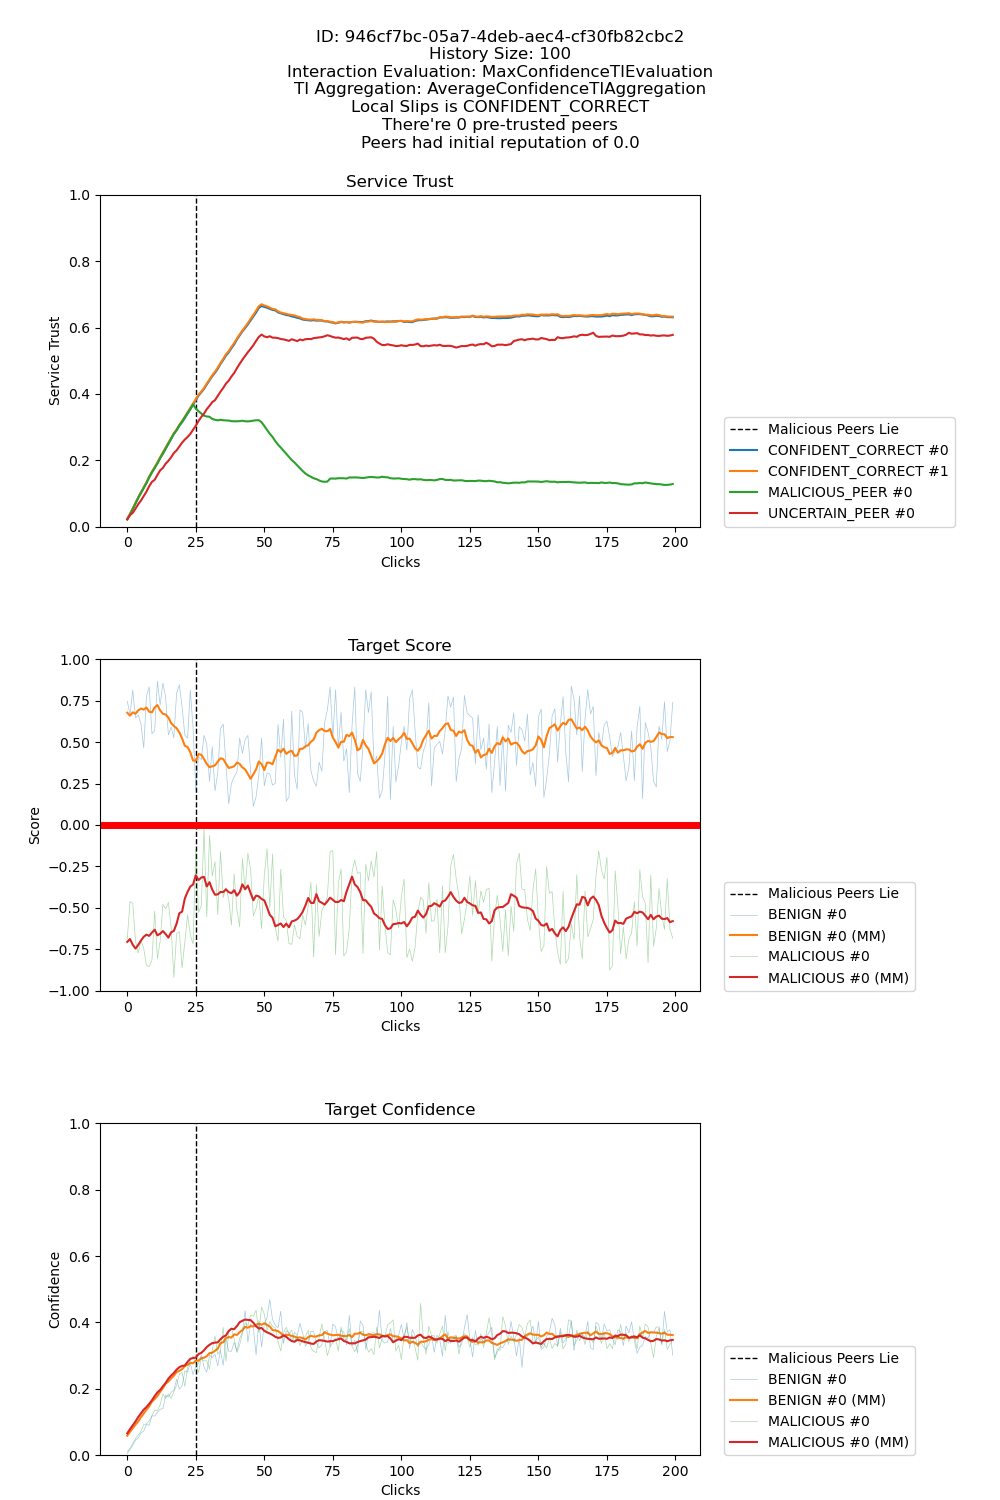
\includegraphics[width=0.83\textwidth]{assets/example_evaluation.png}
    \caption{An example outcome from a single simulation. The graph on top shows how \textit{service trust} changes as time goes by. In this example there are four peers, two confident correct, one uncertain and one malicious. The graph in the middle shows the score for the targets as computed by Fides based on what the peers said. There are two targets (imagine \textit{google.com} and \textit{evil.com}) and Fides computes the score for each of them: 1 means benign, -1 means malicious. The lower graph shows the aggregated confidence for the same targets. That means how confident is Fides about the score in the middle graph.}
    \label{fig:single-simulation-example}
\end{figure}

The graph's headline explains which setup parameters were used for the trust model. In the case of Figure~\ref{fig:single-simulation-example} Fides used the interaction evaluation strategy $MaxConfidenceTIEvaluation$ (Section~\ref{subsec:MaxConfidenceTIEvaluation}).
For aggregating threat intelligence, Fides used the aggregation described in Section~\ref{sec:network-intelligence-aggregation}.
The local Slips instance behaved like a confident correct peer outlined in Section~\ref{subsubsec:confident-correct-peer}.

The graph on top in Figure~\ref{fig:single-simulation-example} shows the development of the \textit{service trust} $st_{i, j}$ (Section~\ref{subsec:service-trust}) on the vertical axis over \textit{time} on the horizontal axis. As mentioned in Section~\ref{sec:environment-simulation}, the time is measured in \textit{clicks}.
The higher the service trust is for a peer, the higher impact it has on the final aggregated threat intelligence.
One can see multiple peers that were involved in the simulation and their respective behavior. All possible behaviors are described in Section~\ref{sec:peers-behavioral-patterns}.
There were four different peers that were communicating with the local instance of Fides, two of them were \textit{confident correct}, one was an \textit{uncertain peer} and the last one was a \textit{malicious peer}.

The dotted line indicates the time when the malicious peers start lying.
One can see that during this first period, when the malicious peers were not lying \textit{(before the line)}, they were gaining the service trust.
In the case of Figure~\ref{fig:single-simulation-example} this happened at click 25 when the malicious peers started lying.
After that, it is clear that they started to lose the service trust.

The second graph in Figure~\ref{fig:single-simulation-example} shows the \textit{target score} during the time (\textit{clicks}).
The target score $S^{k}_{T}$ (Section~\ref{sec:network-intelligence-aggregation}) is the part of the aggregated network threat intelligence, that was computed from the scores and confidences provided by each peer.
The score was calculated by Fides at click $k$ for target $T$.

The score graph contains two different targets, one that is according to the ground truth malicious and a second one that was benign.
We also included the moving average value (indicated as MM) within the window of 10 clicks to make the graph clear.

Finally, the third graph, displays the aggregated confidence $C^{k}_{T}$ (Section~\ref{sec:network-intelligence-aggregation}) over time (\textit{clicks}).
The graph is similar to the score, we include raw values for each time window and target, as well as the moving average within the window of 10 clicks.

In this example output graph, it can be seen that Fides was clearly able to identify that the malicious peer started to lie after click 25 because of the service trust $st^{k}_{i,j}$ for this peer that fell down almost instantly.
At the same time, we can see that on the score graph, the $S^{k}_{T}$ for both targets were skewed and started to get closer to $0$ because the malicious peer had already gained service trust and thus the threat intelligence provided by it had an impact on the final $S^{k}_{T}$.
However, after Fides identified that the peer is lying, it lowered the service trust for this peer, and the score started to recover closer to the baseline.

\section{Evaluation of Fides Resilience in Different Scenarios}
\label{sec:fides-resilience}

To evaluate the resilience of Fides in different scenarios, we need to find the optimal configuration for the following parameters in Fides: interaction evaluation strategy (Section~\ref{sec:interaction-evaluation-strategies}), threat intelligence aggregation function (Section~\ref{sec:network-intelligence-aggregation}) and initial reputation (Section~\ref{subsubsec:computing-reputation}). Each combination of parameters is evaluated in its capacity to correctly classify targets in \textit{any} network topology.\footnote{Distribution of correct/uncertain/incorrect/malicious peers in the network.}
In other words, what setup should the Fides's administrator use in order for Fides to guarantee that it will be able to \textit{eventually} classify targets correctly.

We discovered that actually there \textbf{exists} a particular setup that guarantees that Fides is able to eventually classify the targets correctly in a very adversarial situation. When Fides communicates with at least 25\% of pre-trusted peers from pre-trusted organizations ($0.25 \cdot |P|$ are pre-trusted) and uses $DistanceBasedTIEvaluation$ (section~\ref{subsec:distance-based-eval}) for evaluating the interactions in combination with $AverageConfidenceTIAggregation$ (Section~\ref{subsec:AverageConfidenceTIAggregation}) for aggregating the threat intelligence; then Fides is able to correctly classify the targets no matter how many adversarial peers are in the network (up to filling the remaining 75\%) or how hard they lie.

\subsection{Correct Target Identification Under Harsh Conditions}
\label{subsec:correct-target-identification-no-matter-what}

The first scenario that was evaluated was when the network has 25\% of pre-trusted peers. Several configurations were simulated, which results are shown in Figure~\ref{fig:performance-all-setups-25-pretrusted}.
There are three rows and four columns. Each row contains a single interaction evaluation strategy (Section~\ref{sec:interaction-evaluation-strategies}) and each column contains a single metric that evaluates the behavior of that strategy in the network.
There are three different metrics that evaluate the performance of the Fides's setup and the last graph displays how many confident correct (Section~\ref{subsubsec:confident-correct-peer}) peers there are in the network.
The horizontal axis in each graph measures the environment hardness explained in Section~\ref{subsec:environment-hardness}.
The vertical axis is different for each metric.

As mentioned previously, there are three different metrics.
The first column is a metric measuring target detection performance~(\ref{subsec:target-detection-performance-metric}), the second is the peers' behavior detection metric~(\ref{subsec:peers-behavior-detection-performance-metric}) and the third column then measures the average service trust $st^{kmax}_{i, j}$ for all peers in the simulation.

The last, fourth, column then contains a graph that displays what percentage of peers in the simulation were confident correct~(\ref{subsubsec:confident-correct-peer}) with respect to the environment hardness value~(\ref{subsec:environment-hardness}).
We include it in the graph to allow better visualization of how does the simulation environment looks like with respect to the peer's distribution.

\begin{figure}[hp!]
    \centering
    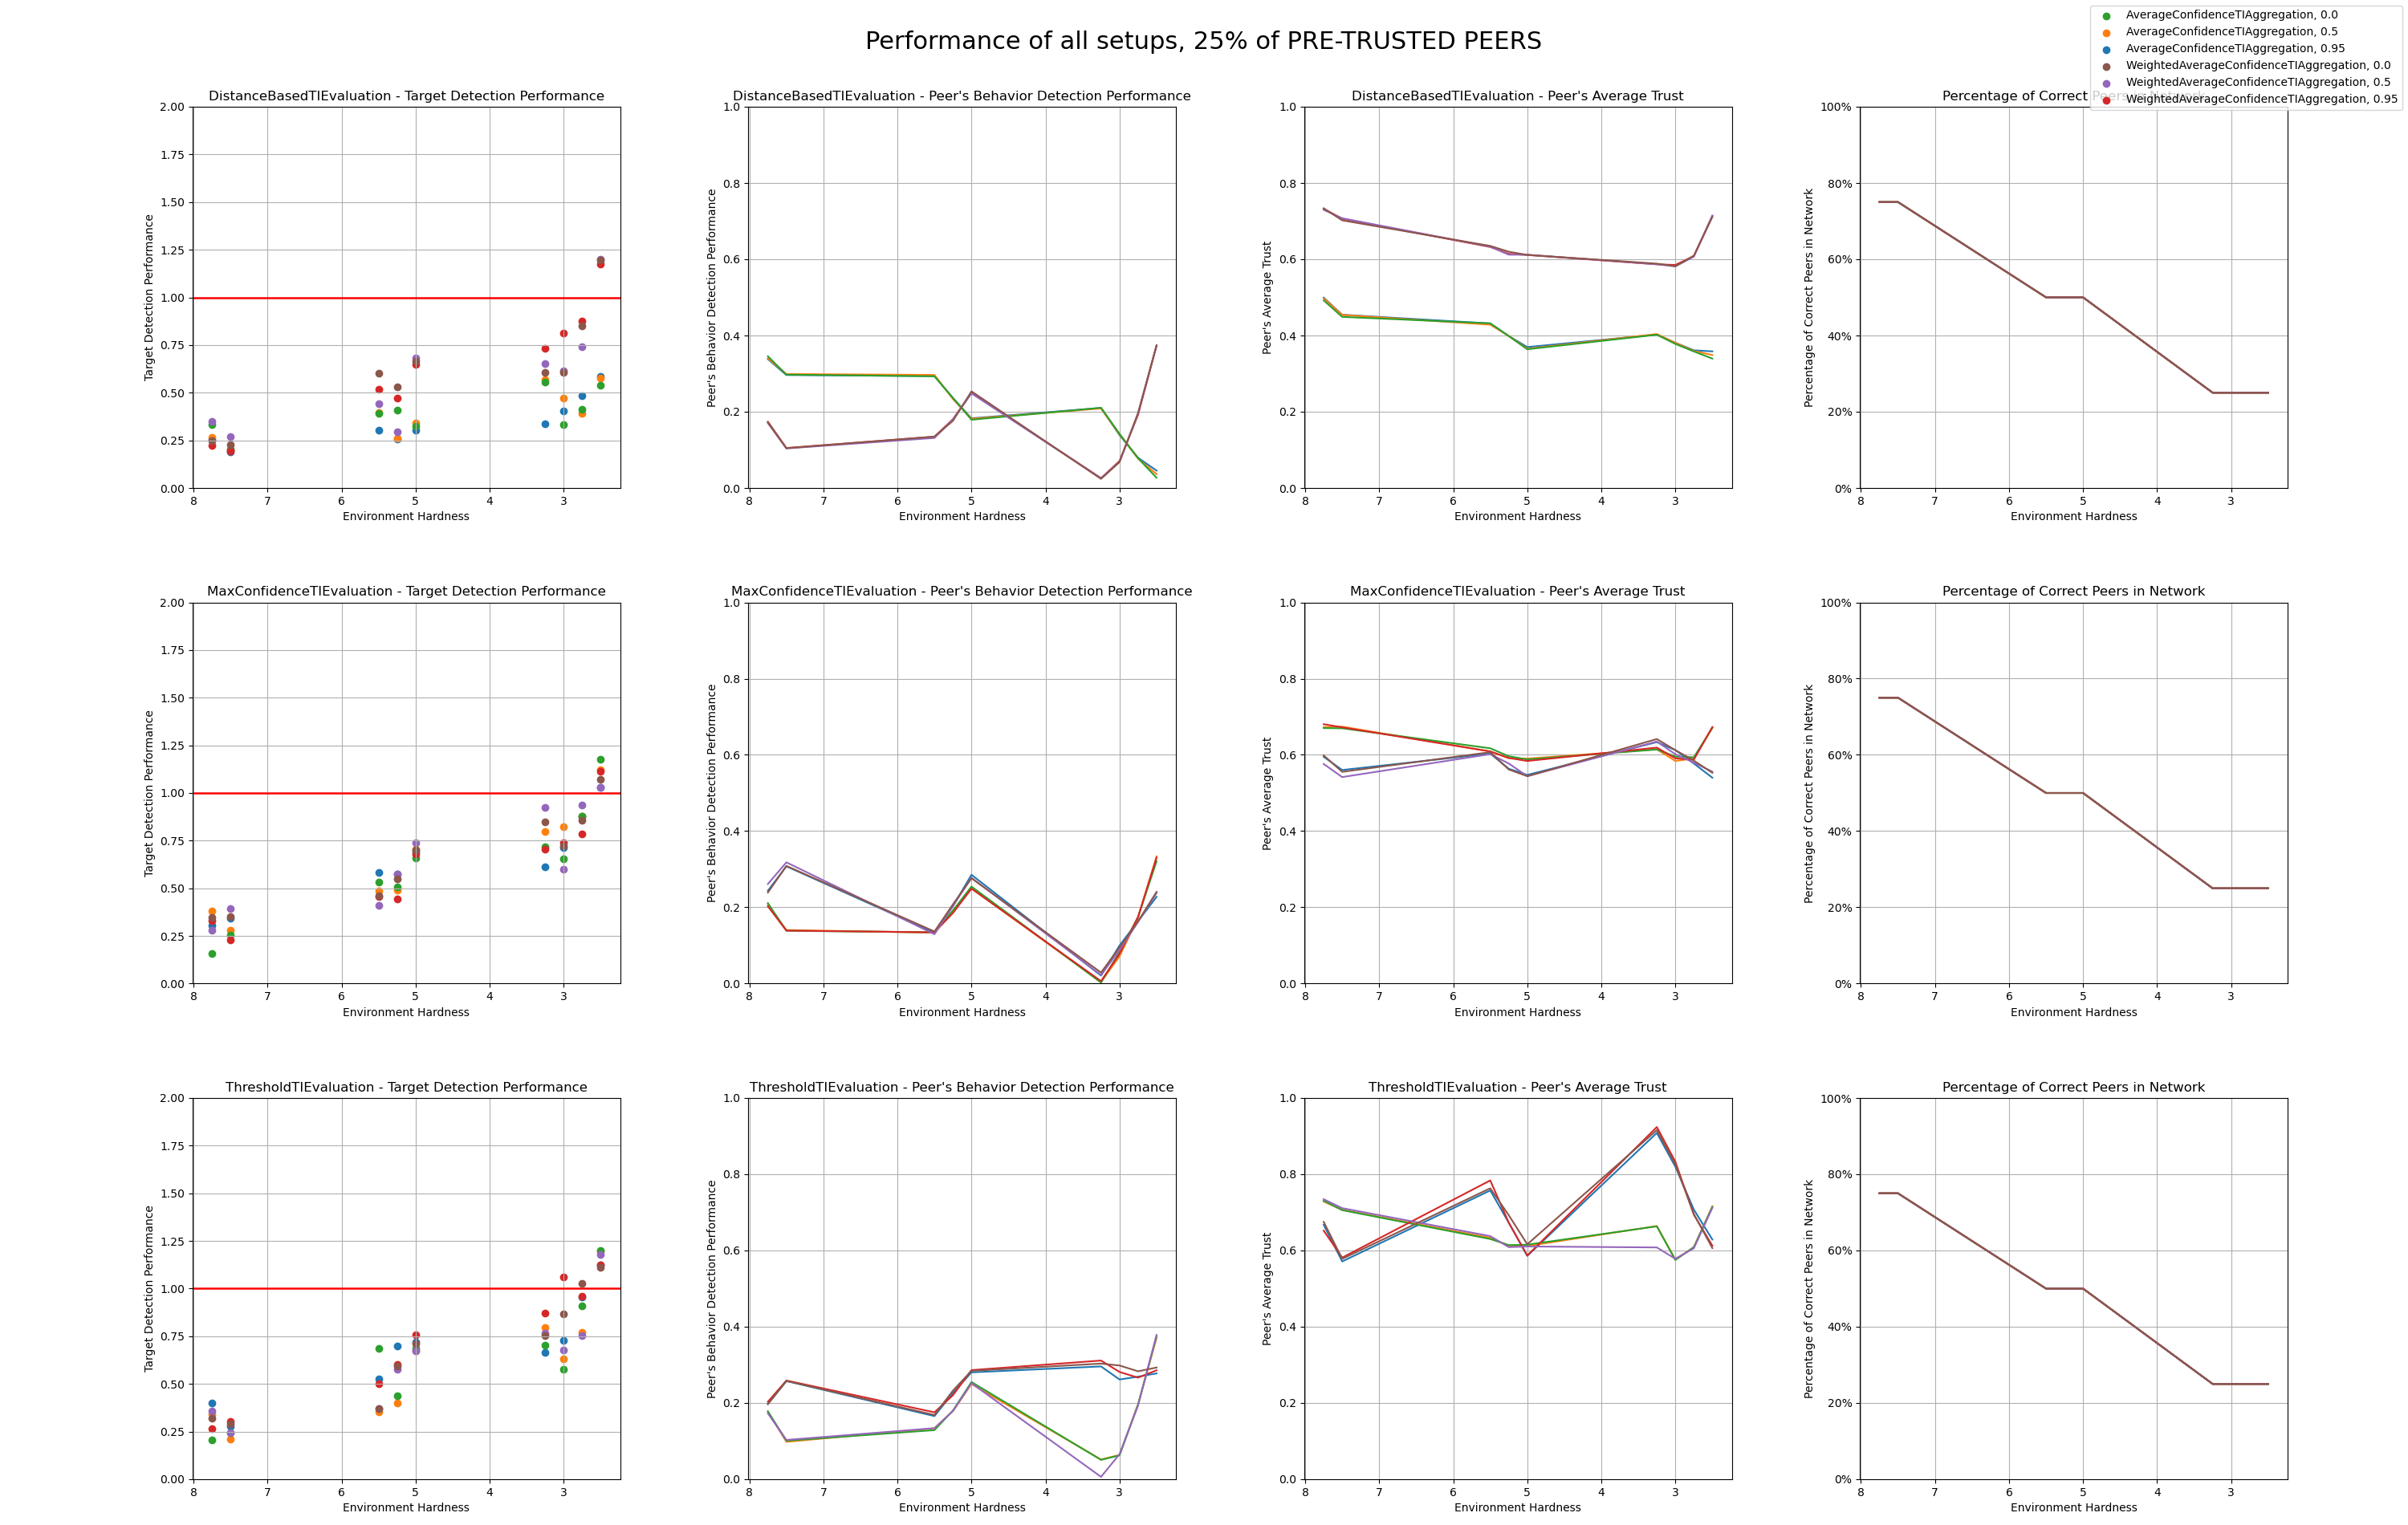
\includegraphics[width=0.94\paperwidth, angle=90]{assets/25_all_metrics.png}
    \caption{Performance of all setups with 25\% pre-trusted peers}
    \label{fig:performance-all-setups-25-pretrusted}
\end{figure}

The most important metric is the target detection performance~(\ref{subsec:target-detection-performance-metric}), which is visualized on the first graph.
A single dot in the graph is the value of $tdp$ and in a case when the $tdp \geq 1$, it means that Fides made on average the wrong decision about the targets and classified them with the wrong label.
In other words, if $tdp \geq 1$, Fides classified benign targets as malicious and the other way around.

\begin{figure}[ht]
    \centering
    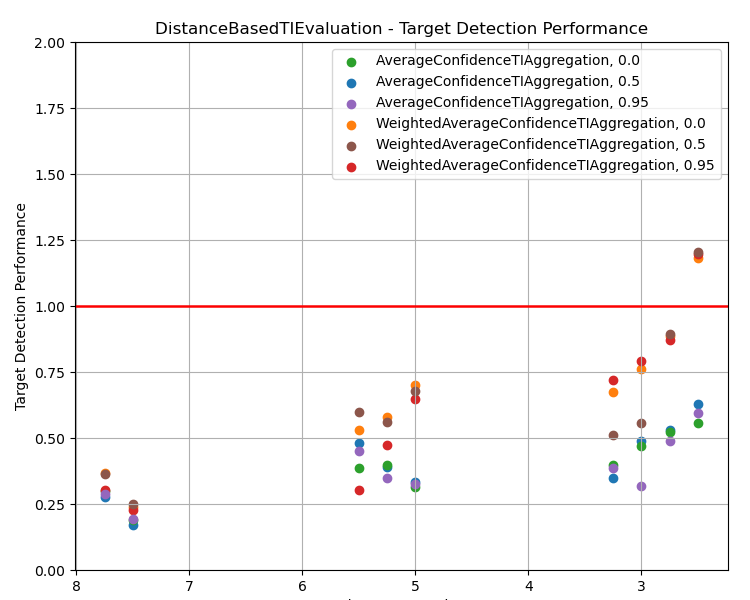
\includegraphics[width=0.7\textwidth]{assets/25_distance_detection_detail.png}
    \caption{$DistanceBasedTIEvaluation$ with 25\% of pre-trusted peers}
    \label{fig:distance-detection-detail-25}
\end{figure}

In Figure~\ref{fig:distance-detection-detail-25} we can clearly see, that there is a situation, even in the hardest environment, where the $DistanceBasedTIEvaluation$ in combination with $AverageConfidenceTIAggregation$ does not have any $tdp$ above the \textit{red line} which means that $tdp < 1$ and that Fides was always able to identify targets correctly even in the worst possible environment.

We included the graph of this case similar to the Figure~\ref{fig:single-simulation-example} with this particular \textit{"winning"} setup in the most hostile environment to the appendix in Figure~\ref{fig:worst-best-scenario}. For the explanation of the graph see Section~\ref{sec:general-overview-of-simulation-output}.

Interestingly, in this particular case, the initial reputation does not affect the final outcome of the simulation, but it does affect the progress as when using an initial reputation higher than $0$, Fides provides wrong scores in the situation when the malicious peers started to lie.
However, it discovers that the peers are lying, which decreases their service trust and is able to eventually recover the correct labels for the targets.
The score value over time for this situation can be seen on the Figure~\ref{fig:missclassification-score-only}.
We included the whole graph in the appendix in Figure~\ref{fig:missclassification-recovery}.

\begin{figure}[ht]
    \centering
    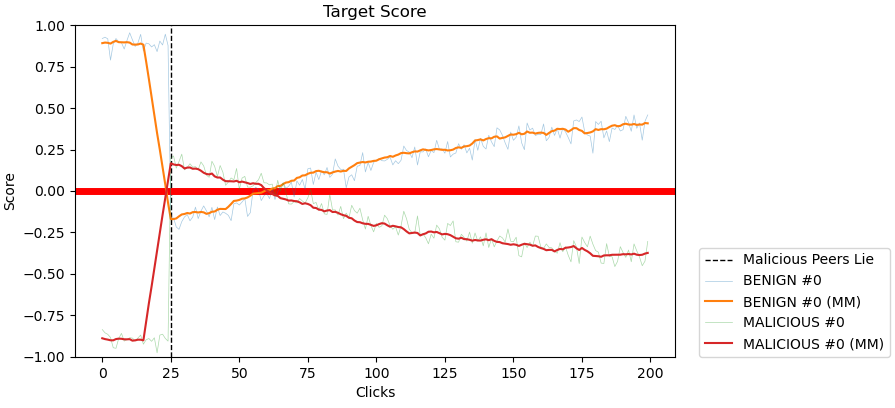
\includegraphics[width=0.9\textwidth]{assets/misclassification_score.png}
    \caption{Score in figure~\ref{fig:missclassification-recovery}.}
    \label{fig:missclassification-score-only}
\end{figure}

It is clear from Figure~\ref{fig:distance-detection-detail-25}, that when Fides used the threat intelligence aggregation method $WeightedAverageConfidenceTIAggregation$~(\ref{subsec:WeightedAverageConfidenceTIAggregation}), it miss-classified the targets in one situation.
Thus, this method does not provide a guarantee that Fides will end up with correct classifications for every target.

The same applies to all other interaction evaluation methods as we can see in the Figure~\ref{fig:performance-all-setups-25-pretrusted} that in the hardest environment, they all classified the targets poorly with all threat intelligence aggregation methods.

\subsection{Resilience Under Different Conditions}
\label{subsec:resilience-under-different-conditions}

We include a similar graph to Figure~\ref{fig:performance-all-setups-25-pretrusted} for the situations with no pre-trusted peers in the appendix in the Figure~\ref{fig:performance-all-setups-0-pretrusted} and then situations with 50\% of pre-trusted peers in the Figure~\ref{fig:performance-all-setups-50-pretrusted}.

With no pre-trusted peers in the network, the results of each configuration vary and they highly depend on the network topology as well as on the knowledge of the local Slips instance.

However, in the case of 50\% pre-trusted peers, one can see that no matter the configuration, Fides was eventually able to determine the correct target classification with a high precision of $tdp \leq 0.7$. Moreover, Fides was able to correctly identify the peer's behavior with the precision of $pbdp \leq 0.2$.

\newpage
\section{Considerations when Evaluating Trust Results}
\label{sec:other-findings}

Even though the results from the previous Section~\ref{sec:fides-resilience} suggest that a combination of $DistanceBasedTIEvaluation$ for evaluating the interactions in combination with $AverageConfidenceTIAggregation$ is the best, there are corner cases where this is not always true.

For example, recall Figure~\ref{fig:single-simulation-example} from Section~\ref{sec:general-overview-of-simulation-output}, where the presented situation uses $MaxConfidenceTIEvaluation$ and it is able to correctly detect all types of peers as well as correctly determine the score for the target.
However, if we take the same environment and the only difference is using $DistanceBasedTIEvaluation$ for evaluating interactions, we get the following graph for the service trust in  Figure~\ref{fig:zero-gained-trust}. The graph for confidence as well as target score for the situation from Figure~\ref{fig:zero-gained-trust} can be seen in the appendix in the Figure~\ref{fig:zero-gained-trust-all}.
This is also the same behavior that we described when we were describing Figure~\ref{fig:0-peer-trust} in the previous Section~\ref{subsec:scenario-with-0-pretrusted-peers}.

\begin{figure}[ht]
    \centering
    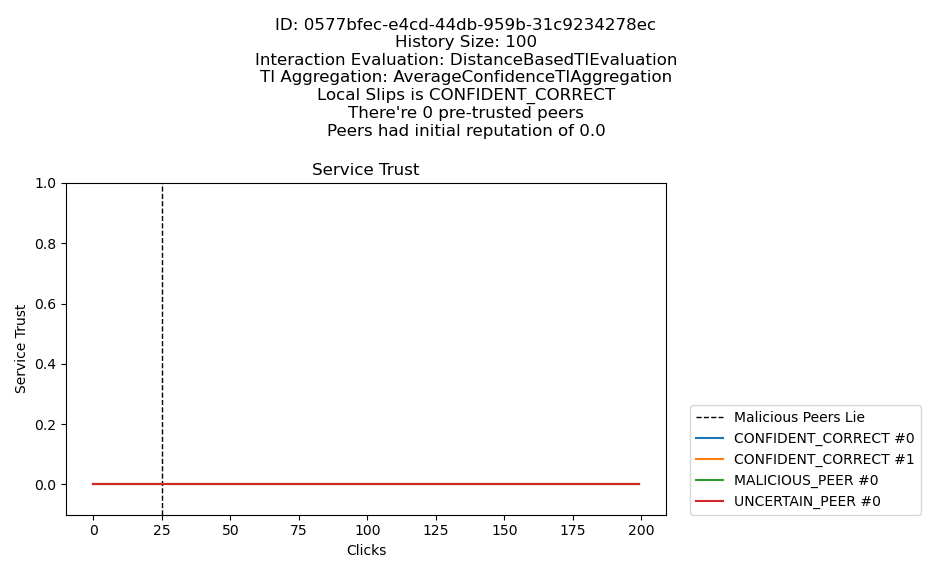
\includegraphics[width=0.8\textwidth]{assets/zero_gained_trust.png}
    \caption{$DistanceBasedTIEvaluation$ in the situation from the figure~\ref{fig:single-simulation-example}}
    \label{fig:zero-gained-trust}
\end{figure}

The service trust graph in Figure~\ref{fig:zero-gained-trust} suggests that Fides didn't gain any trust for any peer in the network.
This happens because the evaluation strategy didn't have enough information at the beginning to evaluate the received data properly.
That leads to peers never gaining any trust and thus not producing any valid outputs because, with no trust, the target score and confidence ended up being $0$ as well.

Another thing to consider is that during the simulations from the previous Section~\ref{sec:fides-resilience}, the local Slips did not know anything about the targets. Which means that whenever Fides requested threat intelligence from Fides, it responded as uncertain peer (Section~\ref{subsubsec:uncertain-peer}). This simulates situations that are close to the reality when Slips is asking about the targets it does not know anything about.
However, it also means that $MaxConfidenceTIEvaluation$ strategy will not live to its full potential as it is also using information from the local Slips. 


\section{Discussion}
\label{sec:discussion}
We discovered that actually there \textbf{exists} a particular setup that guarantees that Fides is able to eventually classify the targets correctly in a very adversarial situation. When Fides communicates with at least 25\% of pre-trusted peers from pre-trusted organizations ($0.25 \cdot |P|$ are pre-trusted) and uses $DistanceBasedTIEvaluation$ (Section~\ref{subsec:distance-based-eval}) for evaluating the interactions in combination with $AverageConfidenceTIAggregation$ (Section~\ref{subsec:AverageConfidenceTIAggregation}) for aggregating the threat intelligence; then Fides is able to correctly classify the targets no matter how many adversarial peers are in the network (up to filling the remaining 75\%) or how hard they lie.

We included the graph of this case, similar to the Figure~\ref{fig:single-simulation-example}, with this particular \textit{"winning"} setup in the most hostile environment to the Appendix in Figure~\ref{fig:worst-best-scenario}. For the explanation of the graph see Section~\ref{sec:general-overview-of-simulation-output}.

\begin{figure}[h!]
    \centering
    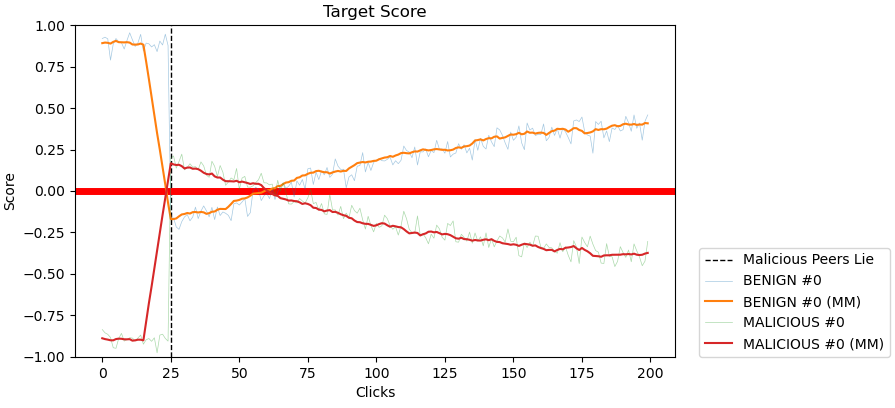
\includegraphics[width=0.9\textwidth]{assets/misclassification_score.png}
    \caption{Score in figure~\ref{fig:missclassification-recovery}.}
    \label{fig:missclassification-score-only}
\end{figure}

Interestingly, in this particular case, the initial reputation does not affect the final outcome of the simulation, but it does affect the progress as when using an initial reputation higher than $0$, Fides provides wrong scores in the situation when the malicious peers started to lie.
However, \textit{in time} it discovers that the peers are lying, which decreases their service trust and is able to eventually recover the correct labels for the targets.
The score value over time for this situation can be seen on the Figure~\ref{fig:missclassification-score-only}.
We included the whole graph in the Appendix in Figure~\ref{fig:missclassification-recovery}.

With no pre-trusted peers in the network, the results of each configuration vary and they highly depend on the network topology as well as on the knowledge of the local Slips instance. The results for the no pre-trusted scenario are shown in Appendix Figure~\ref{fig:performance-all-setups-0-pretrusted}.

In the scenario of 50\% pre-trusted peers, no matter the configuration, Fides was eventually able to determine the correct target classification with a high precision of $tdp \leq 0.7$. Moreover, Fides was able to correctly identify the peer's behavior with the precision of $pbdp \leq 0.2$. This is a very favorable situation for the administrator, where you trust the peers so much that it is not possible for the adversarial peers to modify the belief. The results for this scenario are shown in Appendix Figure~\ref{fig:performance-all-setups-50-pretrusted}.

\bigskip
In general, for a case with no pre-trusted peers and organizations one should use $ThresholdTIEvaluation$ because it proved to be slightly better than the others. However, in cases when the local Slips instance is has some local knowledge about the targets the $MaxConfidenceTIEvaluation$ might be a better choice.

For cases where the Fides communicates with some pre-trusted peers, one should employ $DistanceBasedTIEvaluation$ threat intelligence evaluaiton strategy in combination with $AverageConfidenceTIAggregation$. 
This combination is even able to guarantee that with at least 25\% of pre-trusted peers, it is able to eventually determine correct threat intelligence for all the targets.
\chapter{Conclusion}
\label{ch:conclusion}
In this thesis, we proposed, designed, and implemented a trust model for distributed multi-agent environments of intrusion prevention systems \textbf{Fides}.
Fides enables threat intelligence sharing in global peer-to-peer networks of Slips agents and allows them to cooperate against malicious actors without compromising the security of the local environment. 
We analyzed previous work and various trust models in the chapter \ref{ch:previous-work-background}.
In the following chapter \ref{ch:trust-model-design}, we proposed and designed a computational model of Fides.
In section \ref{sec:attack-vectors}, we described common attacks on the trust models in general and analyzed possible attack vectors for Fides.
The architecture and implementation of the trust model are then described in the chapter \ref{ch:architecture}.
We designed extensive test scenarios and executed 165 890 different test cases in the chapter \ref{ch:experiments}.
Experiments and the trust model itself were then evaluated in the chapter \ref{ch:results}.


\section{Discussion}
\label{sec:discussion}
here we want to speculate a bit about what we achieved and what is great\todo{write this}

\section{Future Work}
\label{sec:future-work}
Even though we achieved our goal of designing a resilient trust model for sharing threat intelligence, there are multiple areas where the model can improve either by exploring different approaches or by implementing new additions to the data flow.

Most importantly, it is clear from the evaluation of simulations in the Chapter~\ref{ch:results}, that Fides performs differently with different setups under different conditions.
Even though we are able to manually pick settings that ensure the best performance, this is not a perfect solution for real-world scenarios.
For that reason, we propose to explore further the following approaches.

\subsection{Exploring Interaction Evaluation Strategies}
\label{subsec:exploring-interaction-eval-strategies}
The trust model developed in this thesis is generic and it is heavily relying on the interaction evaluation function.
This means that the performance of the trust model is as good as the evaluation function.

In this work, we explored evaluation methods that are using only data from a single time window to evaluate the interactions.
However, the local peer might store the complete interaction history with all other peers and whenever it finds out that some peer reported threat intelligence, that proved to be correct after some time, the reporter's service trust should benefit from such discovery.
Another way might be storing the whole interaction history and using machine learning techniques, to discover irregularities in provided data during all communication windows.

In other words, all interaction evaluation strategies described in the Section~\ref{sec:interaction-evaluation-strategies} do not utilize the knowledge from the past, or the history of the interactions.
We believe that this is an interesting space to explore more as it might lead to better performance of Fides in real-world scenarios.

\subsection{Exploring Threat Intelligence Aggregation Methods}
\label{subsec:exploring-threat-intelligence-aggregation-methods}
No threat intelligence aggregation methods explored in this thesis, described in the Section~\ref{sec:threat-intelligence}, use any other information than ones provided by the network at a single time window.
By incorporating information from the recent history, the aggregation might improve the overall detection performed by the trust model.

Moreover, there might be better ways how to aggregate the threat intelligence, or maybe the combination of multiple approaches to one might improve the final confidence in trust model decisions.
As we saw in Chapter~\ref{ch:results}, the combination of interaction evaluation and threat intelligence aggregation influences the performance of the trust model to great extent.

\subsection{Possible Mitigation of Sybil Attack}
\label{subsec:possible-mittigation-of-sybil-attack}
When analyzing the possible attack vectors for Fides, we described the Sybil attack in Section~\ref{subsec:whitewashing-and-sybil-attack} and we stated that Fides is vulnerable to this type of attack.
However, results shown that this is true only in cases when the attacker owns more then 75\% of the network. 
If the attacker controls 75\% of the network and less, Fides has a way how to defend itself and make the correct decisions about the threat intelligence.

There are essentially two possible ways how to mitigate this type of attack even for cases where the attacker controls more then 75\% of the network.

One option is to introduce restriction to Fides, where it uses data at most from the 75\% of peers that are not pre-trusted and the rest, 25\% comes from the pre-trusted peers and organizations. All other data 
That would ensure that Fides always considers only limited amount of data so it will not be vulnerable to an attacker who controls more then 75\% of the network.

The second possible solution would be making it \textit{computationally hard} for new peers to join the peer-to-peer network or generate a new peer identity.
So the attacker would need to spend either time or computational resources when generating new peer identities.
This directly does not prevent a malicious actor to perform this type of attack, but it makes it significantly harder.
However, this mitigation would need to implemented in Iris instead of Fides.

\subsection{Adding Threat Intelligence Challenges}
\label{subsec:adding-threat-intelligence-challenges}
Fung et al~\cite{fung2008trust} explores an interesting idea of creating initial trust in remote peers by giving them \textit{computational challenges}.
In our case, challenges might be asking the remote peer for threat intelligence about the target, that the local Slips know very well and with high confidence.
When the trust model receives a response it uses the interaction evaluation strategy described in the Section~\ref{subsec:use-local-threat-to-evaluate} to evaluate the received data.
The trust model can then ask multiple times to have more interactions and thus effectively \textit{probing} the remote peer and getting an estimate about its future behavior.

By using this approach, one can either replace the recommendation system or greatly improve it in cases when the trust model does not have enough pre-trusted peers.
The disadvantage might be a higher amount of messages sent across the network when the new peer is registered by the network, which could eventually lead even to a denial of service attack on the newcomers. 

This method should be explored more in detail and as the Fides is quite flexible, it can be easily incorporated into the trust model as well.

\subsection{Threat Intelligence Sharing Motivation}
\label{subsec:threat-intelligence-sharing-motivation}
The designed peer-to-peer network for threat intelligence sharing unfortunately does not promote data sharing at all.
The peers sharing threat intelligence are not gaining any benefit other than gaining trust in the eyes of other peers.
As the gained trust brings little to no benefit by itself, there is a lack of incentive for the peers to share their threat intelligence with the network.

However, we can see data and threat intelligence filtering as one of the ways how to motivate other peers to share their threat intelligence.
As we described in the Section~\ref{subsec:data-filtering}, the Fides administrator can choose what threat intelligence is shared with which peers by configuring confidentiality levels with required service trust.
Using this approach, the threat intelligence is shared only with high trusted peers.
That would result in an incentive for the peers to gain the service trust which they do by sharing their own threat intelligence with the network.

Another approach is exploring the idea of \textit{payments} for the threat intelligence where the peers use some sort of cryptocurrency to \textit{pay} for the received threat intelligence and they receive payments for their own threat intelligence they shared.
This would give the peers an incentive to share the threat intelligence and ask for it only when they need it.


% Add bibliography content
\pagebreak
\pagestyle{plain}

\chapter*{Bibliography}
\printbibliography[heading=none]

\cleardoublepage

\pagestyle{fancy}
\chapter*{Appendix}
\stepcounter{chapter}

\begin{figure}
    \centering
    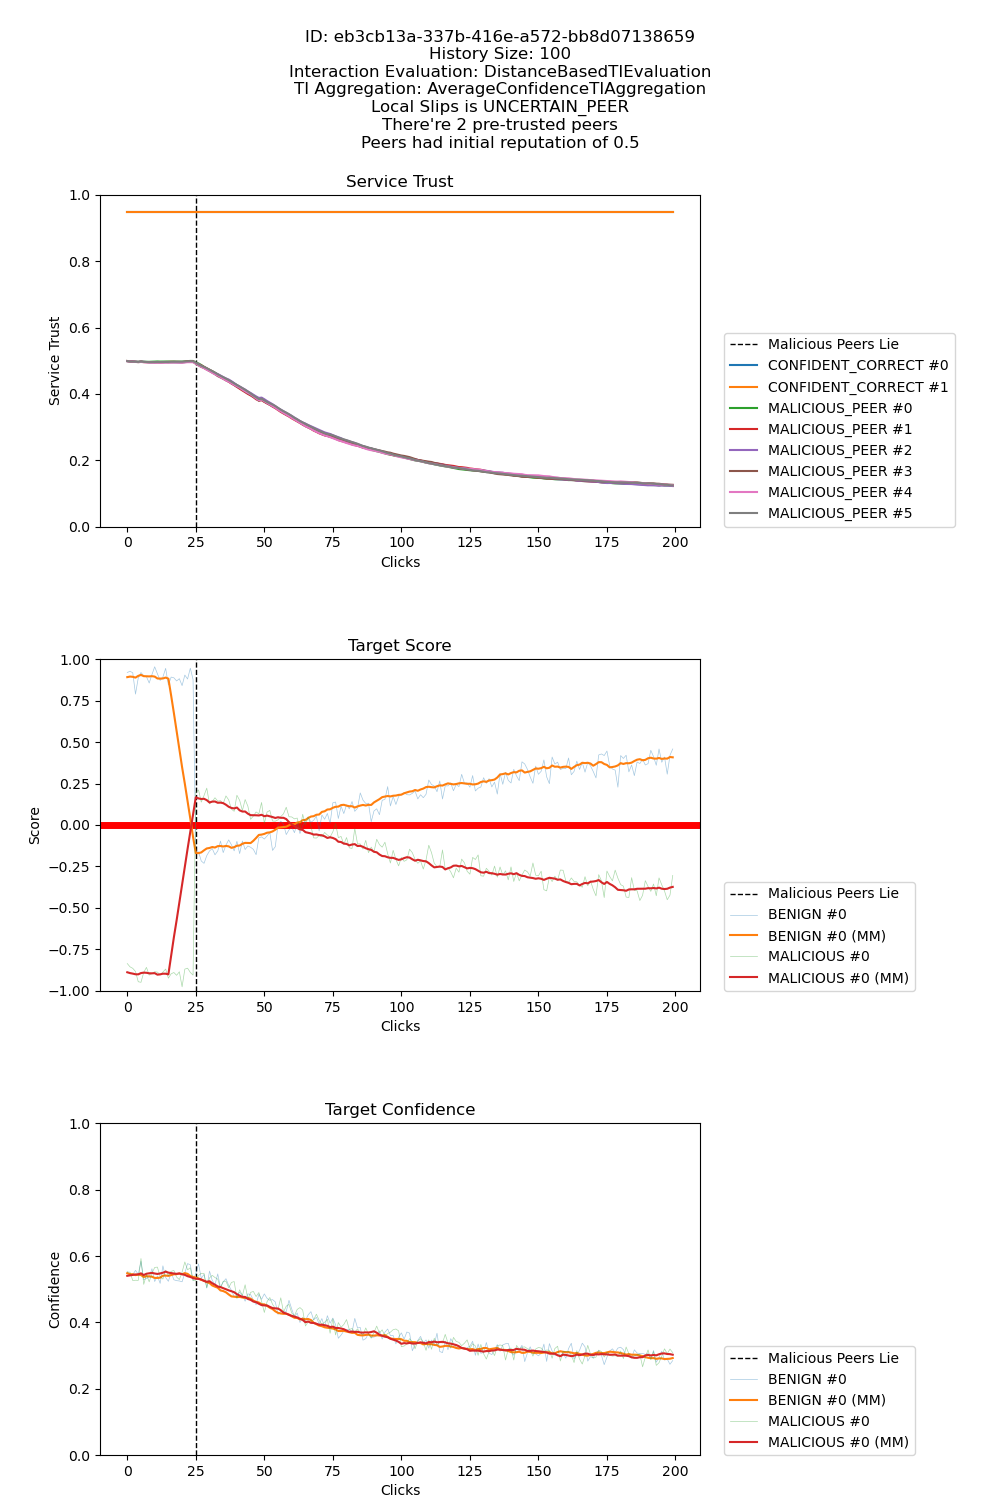
\includegraphics[width=1.0\textwidth]{assets/miss_classification_recovery.png}
    \caption{A scenario described in section \ref{subsec:correct-target-identification-no-matter-what} with initial reputation 0.5}
    \label{fig:missclassification-recovery}
\end{figure}

\begin{figure}
    \centering
    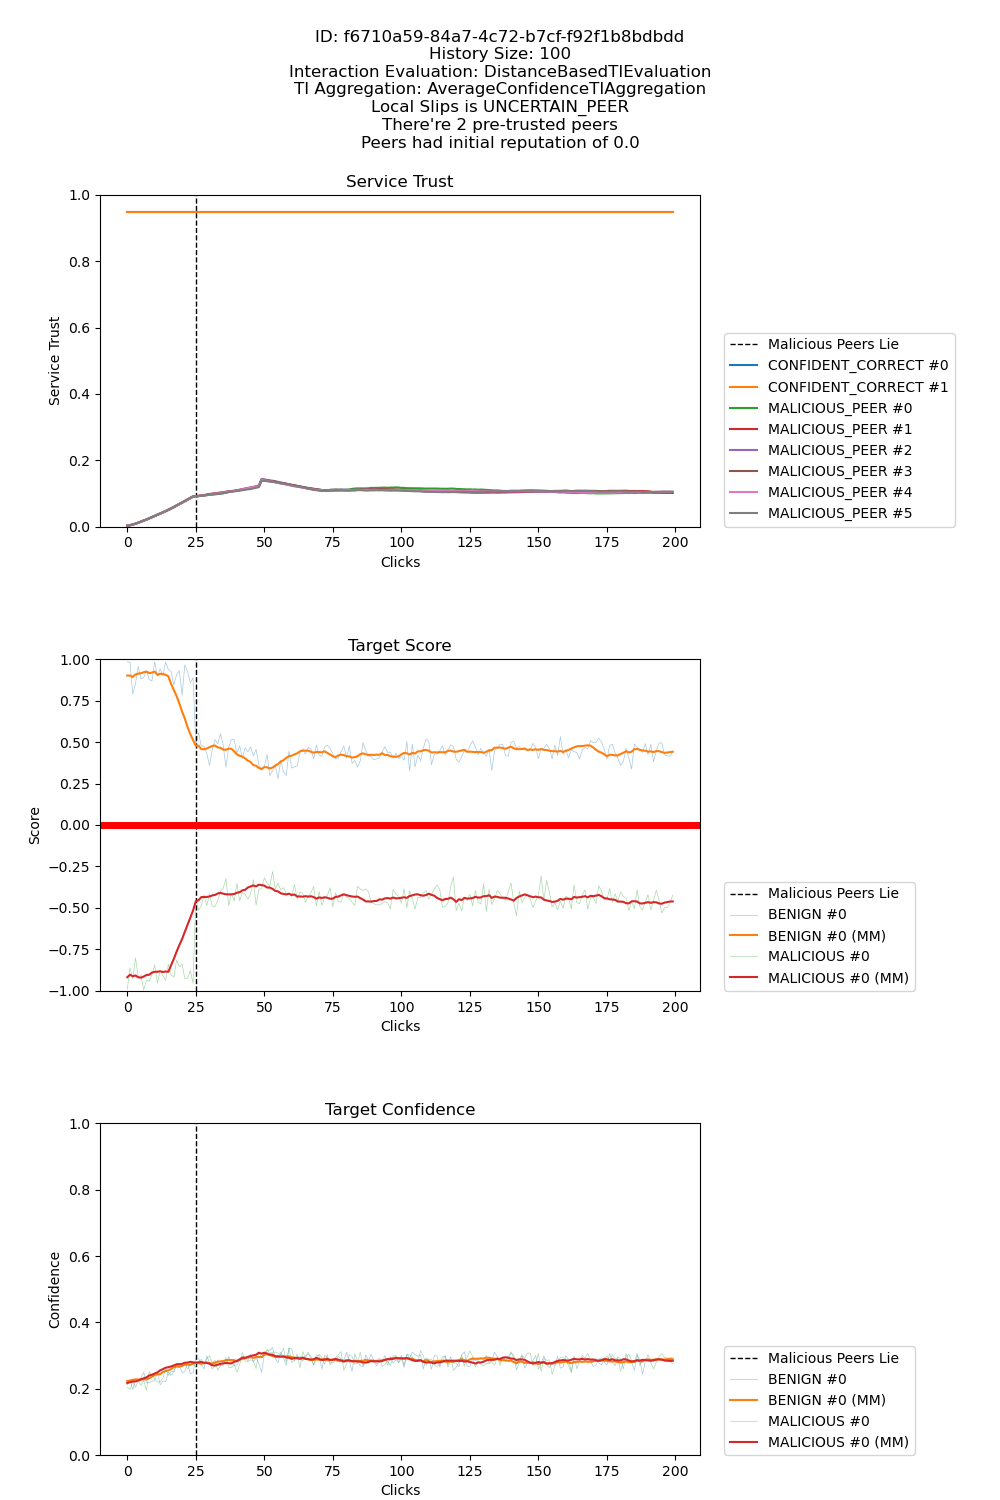
\includegraphics[width=1.0\textwidth]{assets/best_worst_case}
    \caption{A scenario described in section \ref{subsec:correct-target-identification-no-matter-what} with initial reputation 0}
    \label{fig:worst-best-scenario}
\end{figure}

\begin{figure}
    \centering
    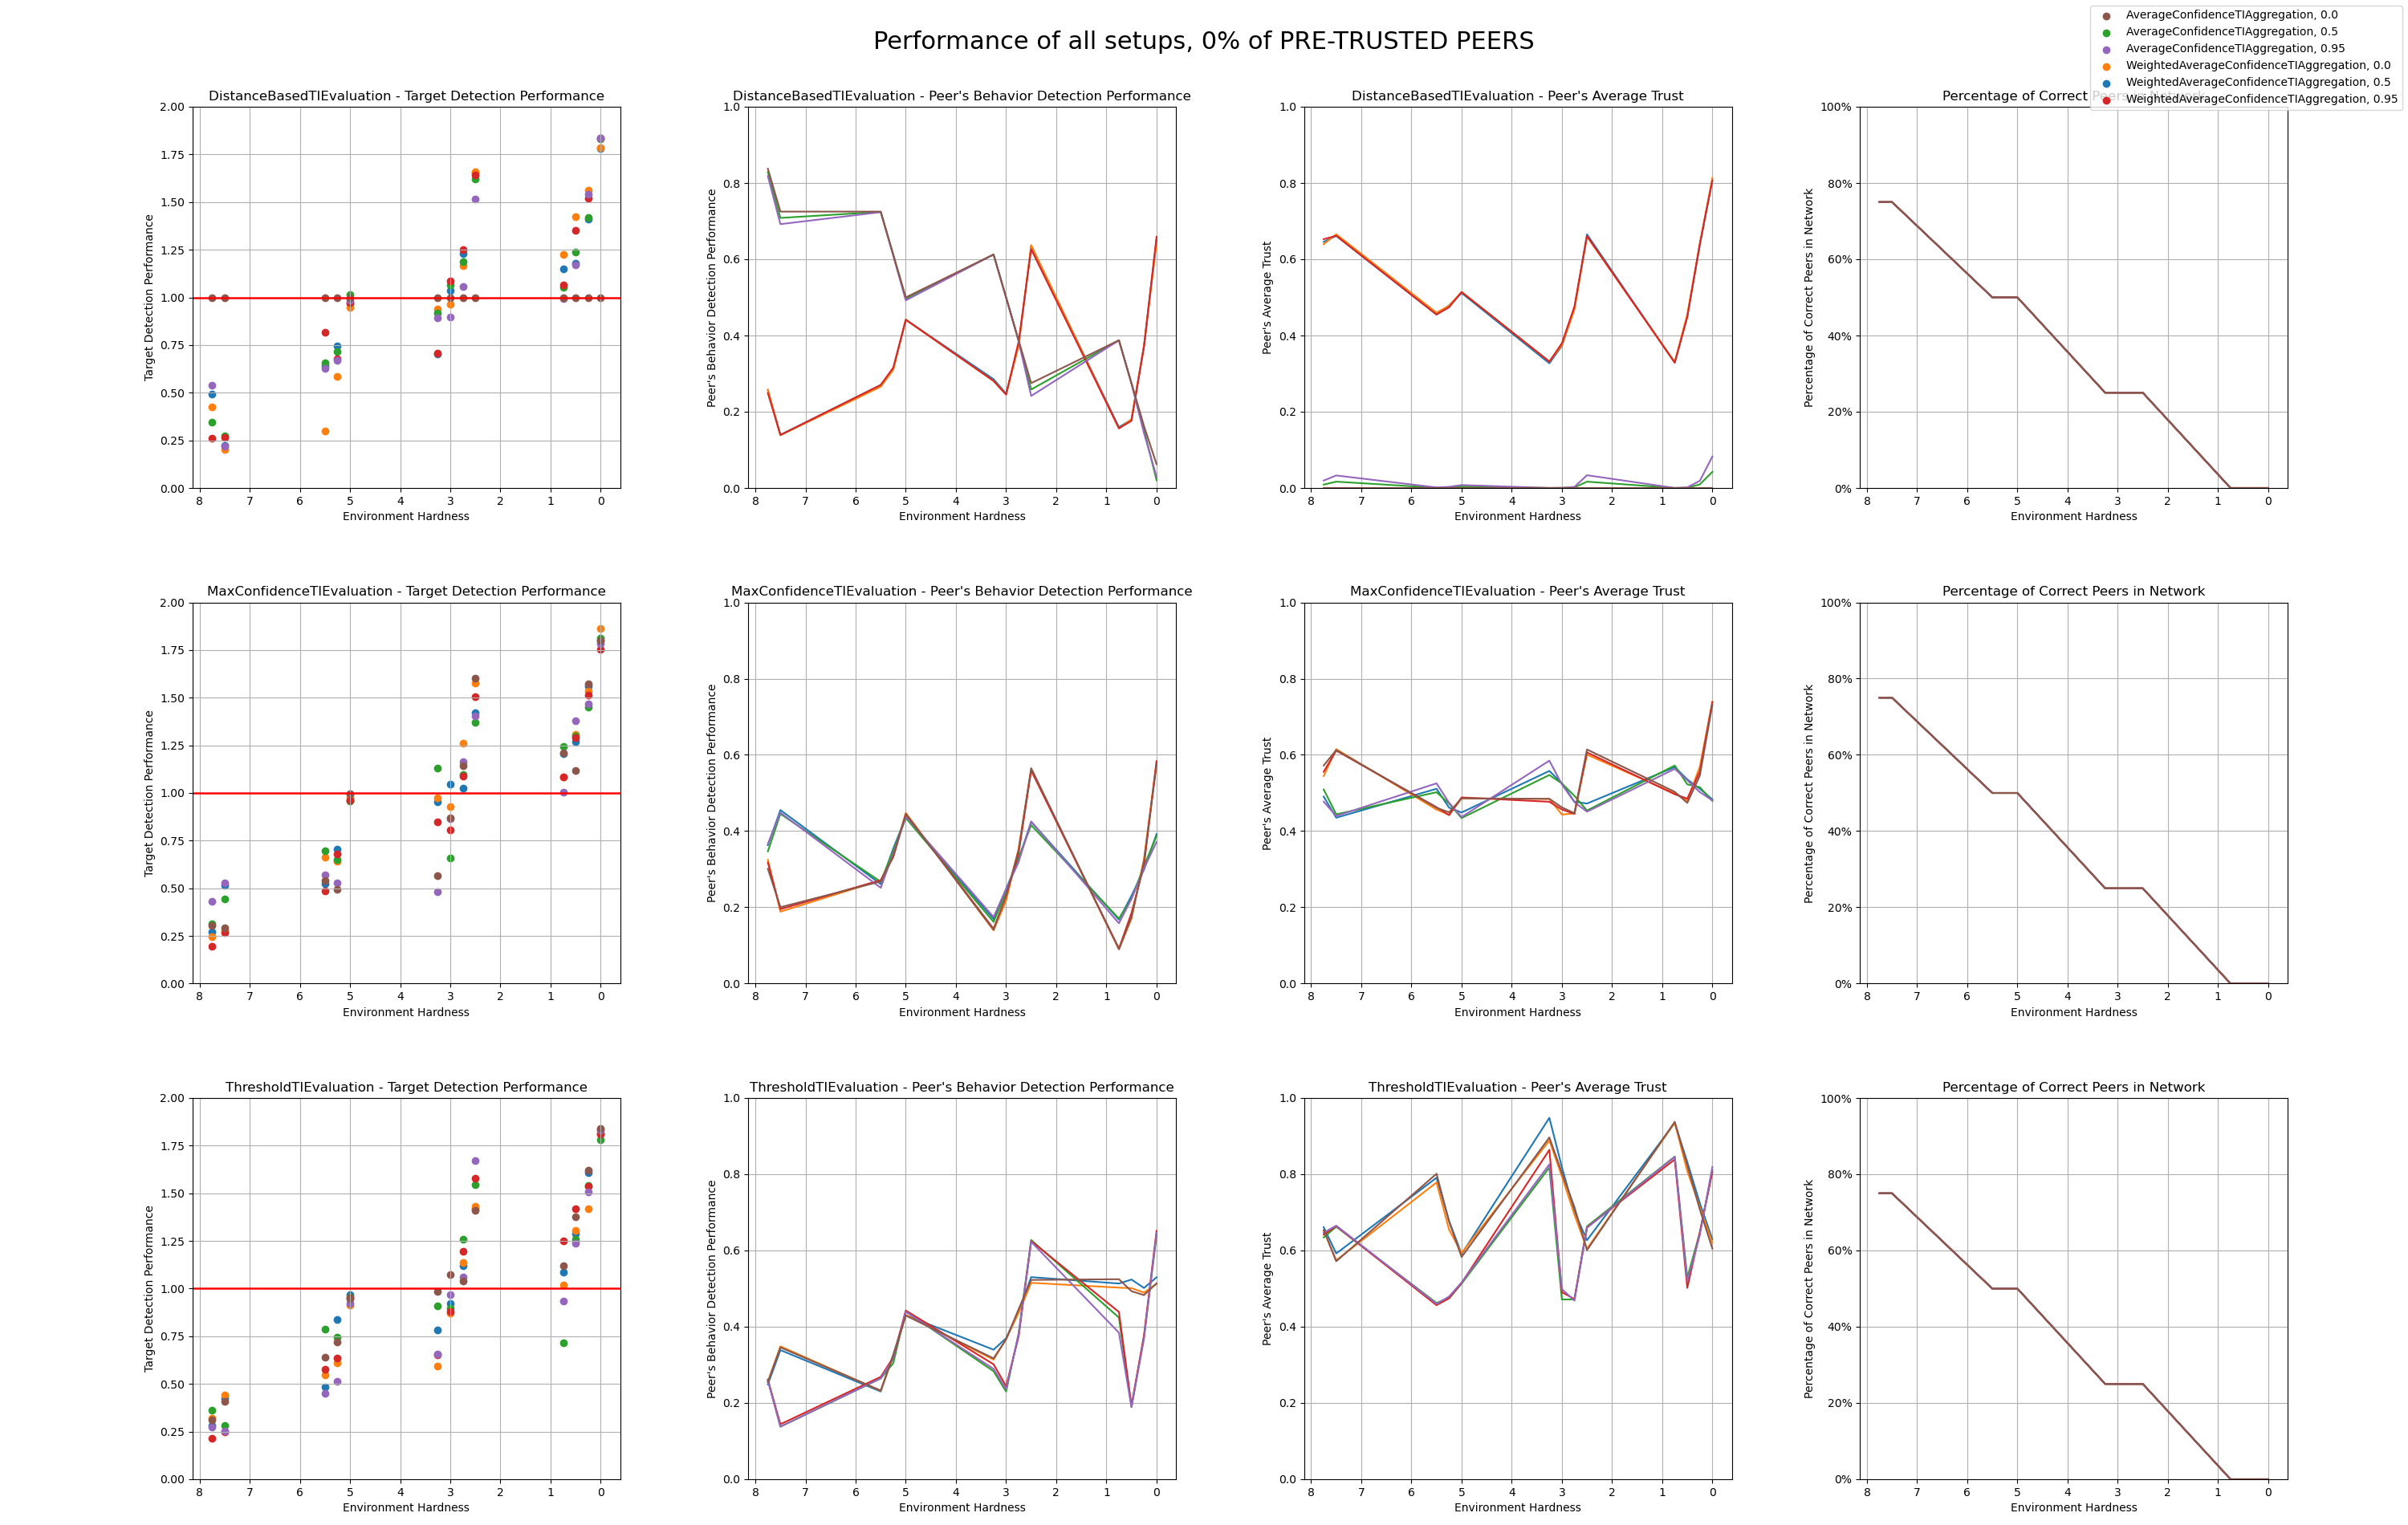
\includegraphics[width=0.9\paperwidth, angle=90]{assets/0_all_metrics.png}
    \caption{Evaluation of performance of all trust model setups with no pre-trusted peers}
    \label{fig:performance-all-setups-0-pretrusted}
\end{figure}

\begin{figure}
    \centering
    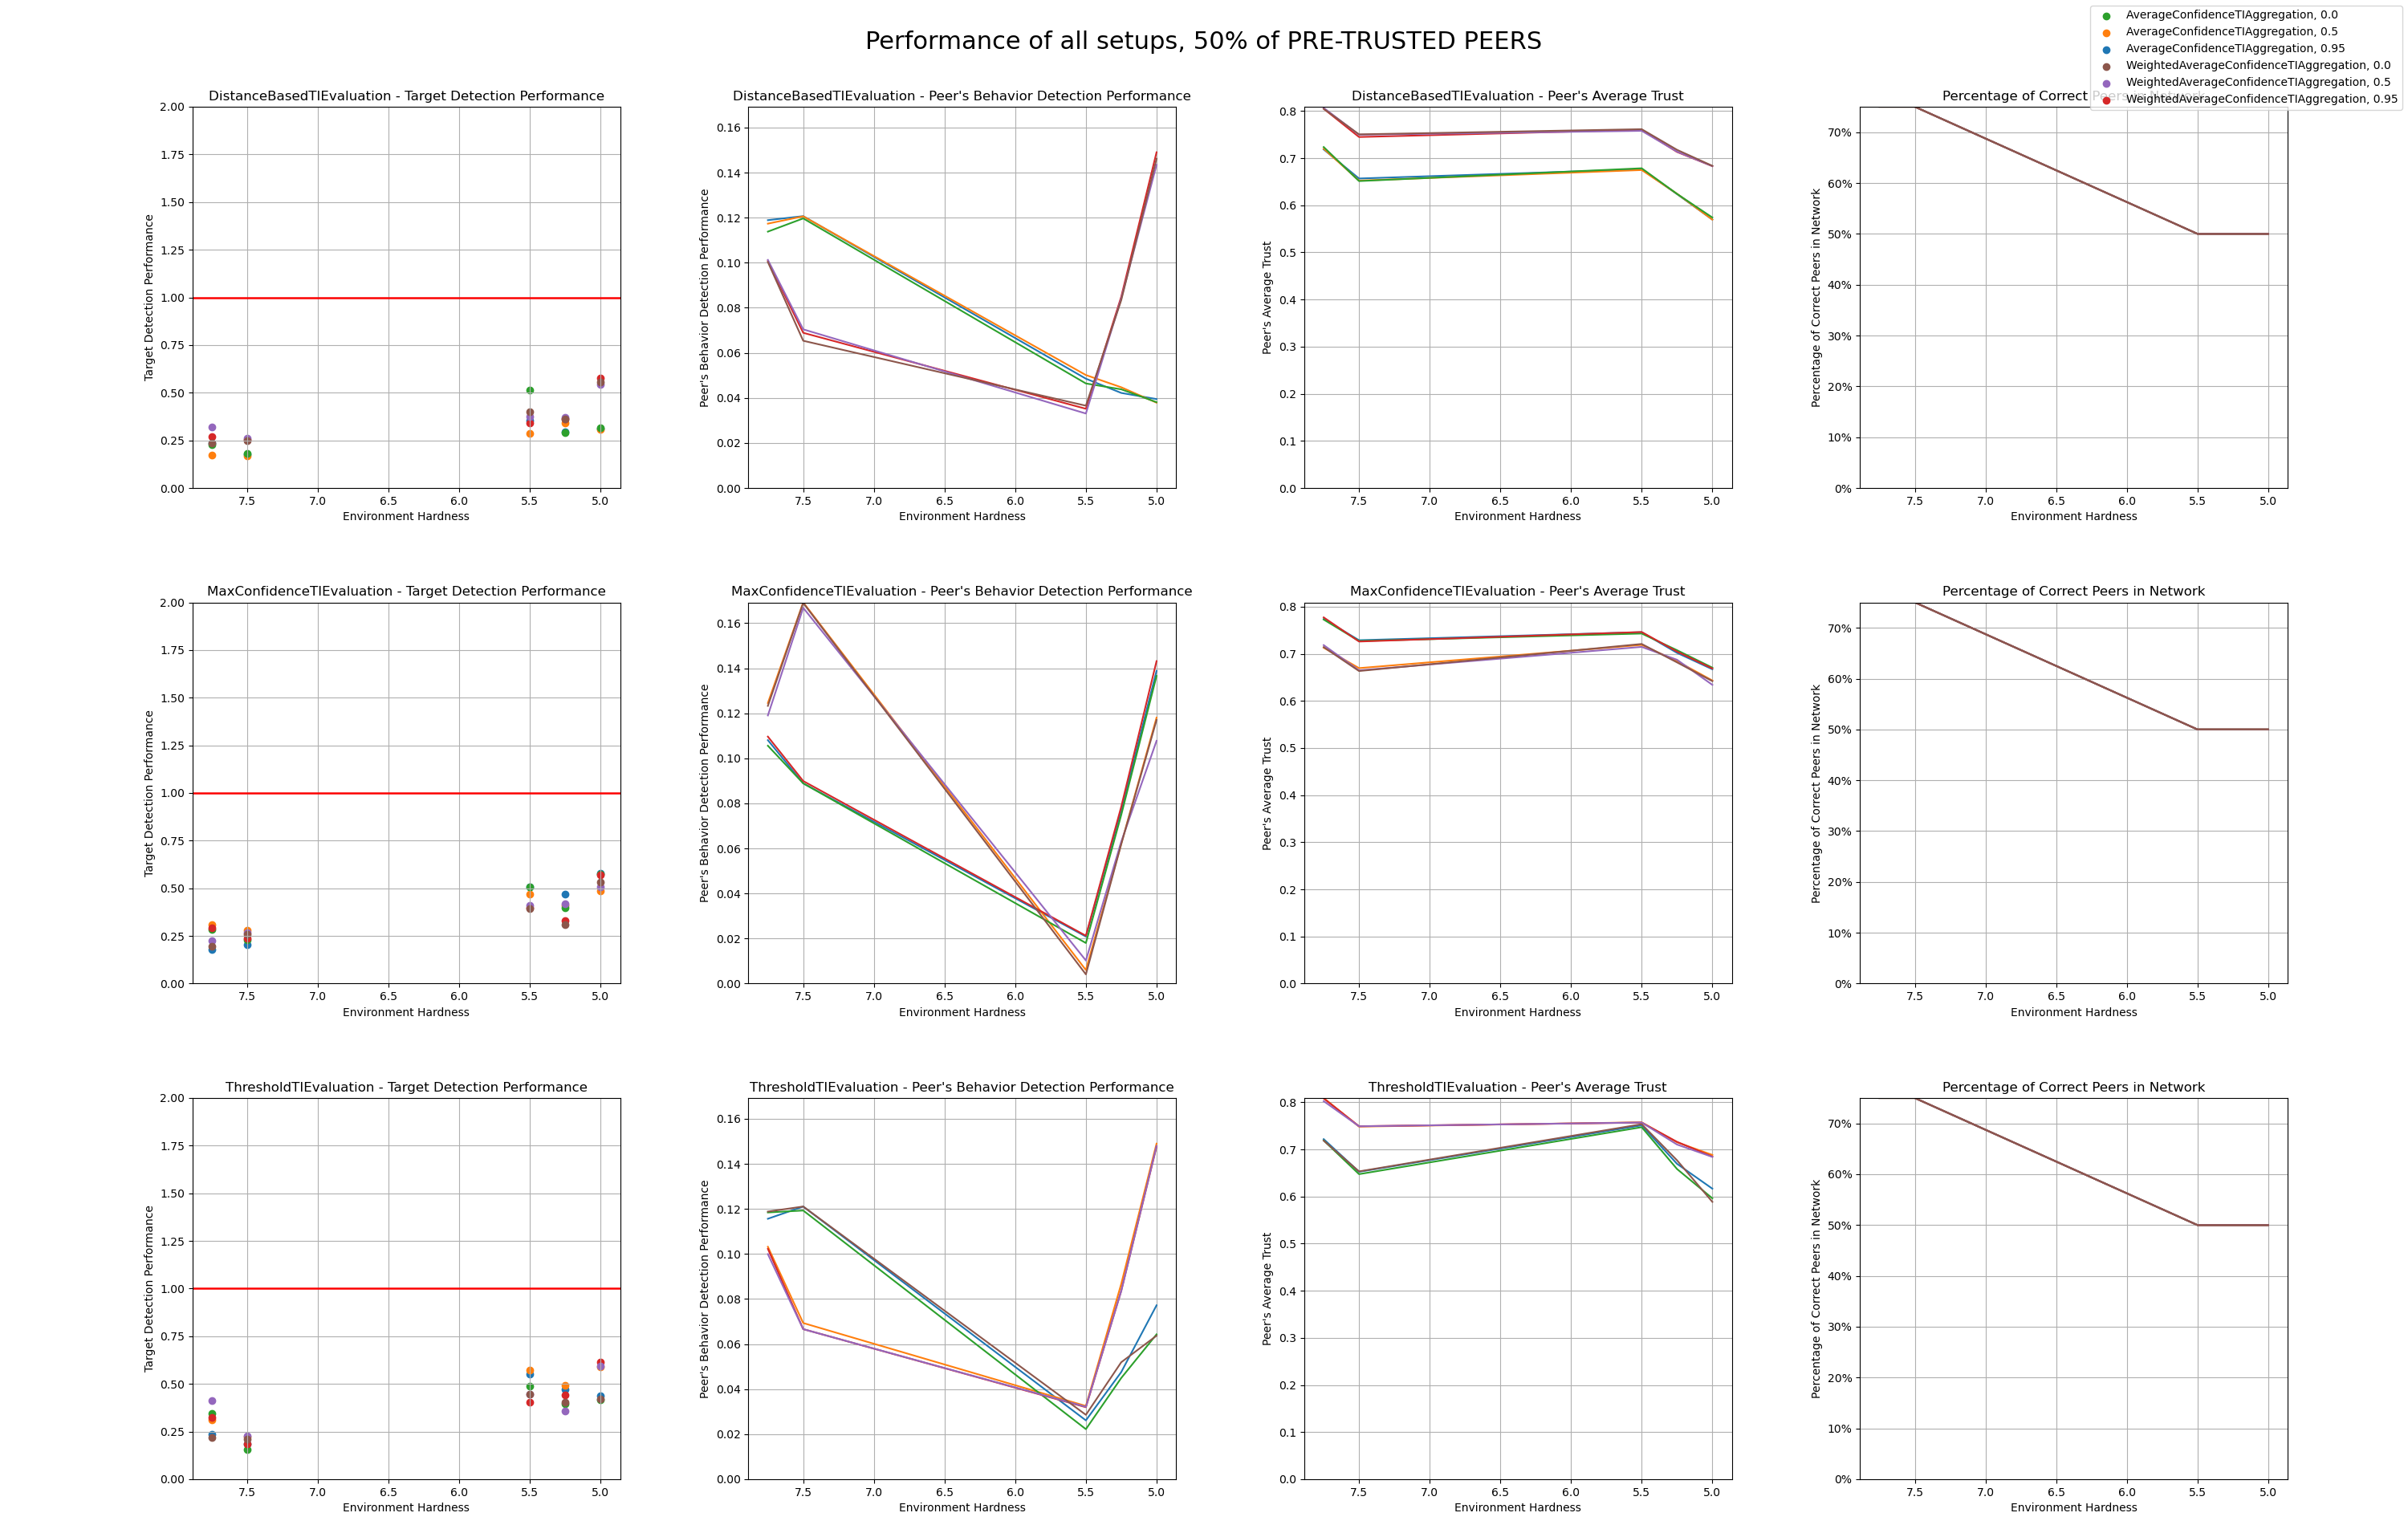
\includegraphics[width=0.9\paperwidth, angle=90]{assets/50_all_metrics.png}
    \caption{Evaluation of performance of all trust model setups with 50\% of pre-trusted peers}
    \label{fig:performance-all-setups-50-pretrusted}
\end{figure}

\end{document}
